\documentclass[11pt,a4paper]{article}
\usepackage[T1]{fontenc}
\usepackage[utf8]{inputenc}
\usepackage{lmodern}
\usepackage[margin=28mm]{geometry}
\usepackage{amsmath,amssymb,amsthm,mathtools}
\usepackage{booktabs,array,tabularx,longtable}
\usepackage{graphicx,tikz}
\usetikzlibrary{arrows.meta,positioning,calc}
\usepackage{enumitem}
\usepackage{microtype}
\usepackage[hyphens]{url}
\usepackage[hidelinks]{hyperref}
\usepackage[capitalize,noabbrev]{cleveref}
\input{glyphtounicode}
\pdfgentounicode=1
\hypersetup{pdftitle={Post-Compromise Security with Persistent Randomness Reservations}}
\newtheorem{theorem}{Theorem}[section]
\newtheorem{lemma}[theorem]{Lemma}
\newtheorem{proposition}[theorem]{Proposition}
\newtheorem{corollary}[theorem]{Corollary}
\theoremstyle{definition}
\newtheorem{definition}[theorem]{Definition}
\theoremstyle{remark}
\newtheorem{remark}[theorem]{Remark}
\setlist{topsep=4pt,itemsep=3pt,parsep=0pt}
\setlength{\emergencystretch}{1.5em}
\newcommand{\artifact}[1]{\texttt{\small\detokenize{#1}}}
\newcommand{\qperiapt}{Q-Periapt Continuity}
\newcommand{\sourcecommit}{\texttt{228c944f}}
\title{Post-Compromise Security with\protect\\ Persistent Randomness Reservations}
\author{}
\date{Research manuscript --- 7 November 2026}

\begin{document}
\maketitle
\begin{abstract}
A persistent messaging protocol can reserve randomness so that interrupted
cryptographic operations can resume with their original inputs. This separates
the creation of secret material from the execution, publication, and confirmation
of the operation that uses it. We study the resulting exposure semantics in a
hybrid post-quantum messaging construction. Our record model assigns immutable
origins to reserved entropy and follows those origins through pending writes,
aggregate images, acquisition, and later wrapping-key disclosure. A
record-interface normalization lemma relates alias-aware storage to an
original-record experiment while preserving acquisition and readability.
For the protocol's multi-epoch symbolic model, a jointly
checked secrecy theorem establishes recovery under fresh target reservations,
unexposed target authentication and entropy, and a precise record-acquisition
condition. Native executions demonstrate the necessity of provenance-sensitive
reasoning: a captured reservation reconstructs later traffic, a reservation
captured during asynchronous confirmation exposes a successor beyond the smaller
confirmation counter, and a
sibling-session write preserves the original secret source. We organize these
results with executable SPQR and whole-KEM reference corpora, and formulate the
common computational experiment needed to connect concrete protected records
to joint root, confirmation, traffic, and acknowledgement security. The analysis
makes the origin and acquisition history of retained secret material explicit
in the recovery statement.
\end{abstract}

\section{Introduction}
\label{sec:introduction}

Post-compromise recovery depends on the secrecy of contributions incorporated
into later keys. Ratcheting protocols make this dependence precise through the
evolution of key-exchange and messaging state
\cite{signal2020,tripleratchet2025}. In a persistent implementation, a
contribution also has a storage history: its randomness is sampled, a replay
record is saved, the cryptographic operation is executed, and its result is
published and confirmed. These events can be separated by a crash or a delayed
message. A security experiment must account for the secret source across this
entire history.

\paragraph{The reservation boundary.}
Consider an endpoint that durably reserves the random tape of a KEM operation
so that an interrupted call can resume with its original inputs. An adversary
acquires this reservation, its wrapping key, and the predecessor root before
the key-generation call executes. After a crash, the endpoint resumes the call
and completes an honestly authenticated exchange. The captured tape determines
the same private key; the public response then determines the KEM contribution
and, with the predecessor root, the descendant traffic keys. The resumed
computation is a later event in the lifetime of the original secret source.

Future-key exposure already has a precise place in messaging security.
SCKA's vulnerable message sets include retained future-epoch keys
\cite{scka2025}, and Triple Ratchet accounts for next-epoch material sampled
while its transmission is in progress \cite{tripleratchet2025}. The question
here concerns the persistent objects from which such material can be recovered:
\emph{which facts about an original operation and the acquisition of its records
must a recovery experiment preserve through restart, copying, and later key
disclosure?}

There are two related difficulties. First, one reservation may occur in a
pending target, a current journal image, and several retained copies. A later
wrapping-key disclosure can make an earlier capture readable, even after the
honest endpoint has deleted its local copy. Second, a cryptographic reduction
may possess a selected operation's public outputs without possessing its
random tape. It must still account for public record commitments, complete-record
equality, exact retries, reached persistence states, and authenticated reports
whose inputs depend on retained private values. These are semantic and
simulation obligations of the recovery argument.

\paragraph{Original sources and durable executions.}
We associate each reservation with its original owner, operation, session,
epoch, and sampling event. We separately identify an immutable session-record
version and a physical image carrying that version. Copying or resealing an
image preserves the referenced source and record version. Acquisition records
the objects obtained by the adversary; readability is evaluated against the
complete acquisition and key-disclosure history. This representation makes
the secrecy premise stable under changes to physical storage representation
while allowing adversarial knowledge to grow.

We study this representation in Q-Periapt Continuity, a hybrid post-quantum
messaging construction with persistent rekey operations and asynchronous
confirmation. The construction provides a concrete setting in which the
reservation, execution, and confirmation events have distinct operational
boundaries. Its journal can also aggregate several sessions, making the
distinction between a new image and an existing source directly observable.

\paragraph{Main result.}
Theorem~\ref{thm:native-online-message} gives confidentiality and fresh-message
integrity for an online selected application send after the next rekey of an
established session, under its finite interfaces and primitive assumptions.
Each endpoint has one authoritative history with passive copies; the network
and recovery schedule remain adversarial. The predecessor
root and wrapping keys may be known. Earlier message keys and the declared
successor values may be disclosed. The target step is selected before its
first private computation at either endpoint, and the terminal selector may
choose the recovery cut after interaction. Eligibility requires both original
KEM reservations to follow that cut, the target signing secret keys and
designated target-epoch entropy to remain undisclosed, and every acquired
target-session version to have been first saved at or before the cut
(\eqref{eq:eligibility}). The theorem bounds the unconditional eligible-message
advantage and fresh-installation event by explicit source-attribution, record,
KEM, shared-oracle key-schedule and AEAD terms. Its executed-slot selector
connects attribution to ordinary hedged ML-DSA security. The first-message and
selected-root confirmation results are established along the same proof route
(Corollary~\ref{cor:live-core-next-rekey} and
Theorem~\ref{thm:native-selected-authentication}).

\paragraph{Technical contributions.}
The construction connects an original-source exposure condition to this
native message experiment through simulatable private retained state.
Reservations keep their original operations, and acquisition is recorded
separately from later readability. Alias normalization preserves the public
view and original-record ledger under copying and resealing
(Lemma~\ref{lem:alias-normalization}). For fixed public key derivations, a
guarded-path characterization exactly matches iterative decryption
(Theorem~\ref{thm:guarded-normalization}). Conjunctive guards capture how
acquired ciphertexts and disclosed keys jointly reveal a source, while
alternative copies provide additional routes to the same source.

The central reduction constructs retained private state around an operation
from its public outputs, while its random tape remains hidden from the simulator.
Images and intents preserve original record identities; dependent immutable
reports are simulated in reverse causal order. Candidate-local accounting
localizes the original native score before comparing each source pair,
using provenance to justify permanent stops for every eventual recovery cut.
The original-operation adapter carries the resulting execution through the
complete ContextBound contribution, root initialization, confirmation and
traffic schedule.

Online message selection requires an additional dependency argument.
Successive Extract and Expand comparisons isolate the selected key while
preserving earlier-key observations, its disclosed successor seed and real
suffix computation. Each comparison retains the first private computation
across endpoint aliases, including failed receive-side advances. The
composition preserves the accepted send's original sources and candidate-local
record stops with explicit lifetime and whole-execution budgets.
Section~\ref{sec:computation} summarizes these allocation boundaries and the
connections supplying the main result.

Component bridges connect operational ML-KEM to ordinary IND-CCA security
through a deferred-challenge comparison, and reserved ML-DSA randomizers to
ordinary hedged unforgeability through a shared-XOF comparison
(Proposition~\ref{prop:kem-deferred-challenge} and
Theorem~\ref{thm:native-mldsa-reservation-bridge}). Joint entry comparisons
retain the multiple uses of a contribution. Complementary bootstrap instances
protect the original inventory source or reply source and establish historical
activation of the complete signed transcript
(Corollary~\ref{cor:bootstrap-initial-terminal} and
Theorem~\ref{thm:bootstrap-terminal}). A further purpose-key instance retains
equal-input aliases and separate returned-owner lifecycles
(Section~\ref{sec:sdk-purpose-connection}).

A mechanized symbolic theorem uses the same provenance condition for message
secrecy across unbounded epochs (Theorem~\ref{thm:symbolic}). Its model includes
inherited roots, shared key identities, alternating proposers and asynchronous
confirmation. Native executions exhibit the exposure distinctions: traffic is
reconstructed from reservations captured before restart; a delayed-receipt
execution exposes epoch-two traffic while the peers' confirmed counters remain
zero and one; and a sibling-session write carries an earlier target reservation
into a new aggregate image.

\paragraph{Supporting validation.}
Independent finite checks validate the guarded characterization under
acquisition, deletion and late disclosure. Source correspondence binds the
native operations to the declared interfaces. Pinned SPQR and whole-KEM
corpora measure reconstructible message sets across schedules. A further 49
native/reference executions share directed transmission opportunities,
charging control traffic and exact retries to the same budget and recording
reconstructed messages, commitments, deliveries, bytes and persistence work.
A one-way control records exhausted-budget suspension. In a paired 28-run
native ablation, a minimum retry age of four public sender turns increases
completed service in every measured bidirectional or resumed schedule while
retaining the alternating current-epoch exposure counts and recording
schedule-dependent communication costs.

\paragraph{Security model and organization.}
Crash recovery resumes retained, bound operations under the authentication,
acquisition and disclosure interface of Section~\ref{sec:security-model}.
The symbolic theorem covers unbounded epochs. The computational results
connect the stated finite record, report and online message interfaces within
the common message experiment, retaining their explicit cryptographic and
disclosure terms. Section~\ref{sec:construction} describes the construction;
Sections~\ref{sec:security-model} and~\ref{sec:computation} develop the record
model and computational connection. Section~\ref{sec:established} presents
the mechanized recovery theorem and separating executions, and
Section~\ref{sec:evaluation} validates the exposure semantics and presents
the matched executions. Section~\ref{sec:discussion} develops their
consequences and further instantiation.

\section{Related work}
\label{sec:related-work}

Our comparison separates the security of a ratcheting construction, the
exposure represented by its state, and the interpretation of that state in a
durable implementation.  This places the reservation problem alongside
existing cryptographic and systems results without identifying a new storage
write, a completed exchange, and a recovered secret as the same event.

\paragraph{Ratcheting and exposure of future messages.}
Cohn-Gordon et al. analyze Signal's X3DH and Double Ratchet core as a multi-stage
authenticated key-exchange protocol \cite{signal2020}.  Their model represents
the branching structure of ratchet stages and specifies admissible key
disclosures for a challenged stage.  This establishes an important precedent
for deriving a precise cryptographic object from a deployed state machine.
The object studied here includes a contribution's recoverable randomness
before its KEM computation, together with the record versions that retain it.
Our witnesses connect these earlier objects to later roots and application
messages.

Auerbach et al. introduce SCKA and vulnerable epoch and message sets
\cite{scka2025}.  Definition~3.2 includes current chains, already produced
future-epoch keys, and pending out-of-order message keys.  Theorem~3.3 gives a
secure-messaging construction from secure SCKA, an appropriate KDF, and AEAD.
Their Section~1.2 explicitly identifies state loss and session handling as a
separate setting.  We use their set-based perspective and investigate how
original reservations and persistent-record acquisition determine exposure at
that representation boundary.  In particular, our delayed-receipt witness is
compared with the state of both directions and their retained contributions,
rather than assigned a universal bound from a confirmed-epoch counter.
% Primary comparison: USENIX Security 2025 paper, Sections 1.2 and 3.1--3.3,
% especially Definition 3.2 and Theorem 3.3.  Future-epoch exposure and
% direction/index-sensitive vulnerable sets are already present there.

The timing of secret generation is itself an established design consideration.
Section~8.5 of Signal's Double Ratchet specification discusses deferring ratchet
key generation until it is needed for sending, thereby shortening a key's
lifetime \cite{doubleratchet2025}.  Our contribution concerns the operational
meaning of that lifetime when a durable reservation fixes the key before the
generation call runs.  An implementation can defer computation while retaining
the original coins.  The relevant freshness event is then the reservation,
and its identity must survive retries and subsequent image writes.

\paragraph{Session handling and state-loss resilience.}
Cremers, Jacomme, and Naska distinguish individual ratcheting sessions from the
conversation assembled by a messaging application \cite{sessionhandling2023}.
Their Signal experiments and Tamarin model show how session selection and
retry behavior permit a clone to remain active, and they analyze two mechanisms
for stronger conversation guarantees.  This is directly relevant to the scope
of our disclosure interfaces: a session label identifies a protocol instance,
whereas shared authentication or wrapping keys can connect several instances.
The Continuity model follows actual key identities, and the aggregate-copy
execution examines a concrete storage relationship between two sessions.

Cremers, Medinger, and Naska subsequently prove incompatibilities between full
conversation PCS and specified state-loss resilience requirements
\cite{stateloss2025}.  Their Definitions~1 and~2 require continued communication
after dynamic or static state loss; the distinction includes losing evolving
communication state and losing persistent identity state.  Our crash/resume
setting retains a bound journal and resumes its original operations under
explicit authentication assumptions.  The recovery theorem states exactly
which reservation, identity, and record-acquisition histories are admissible.
Thus, the retained state and independent authentication in our claim identify
the particular recovery setting being studied.  The delayed-receipt and
aggregate-copy witnesses explain how that setting behaves during honest
asynchronous progress.
% Primary comparison: Cremers--Medinger--Naska, Sections 3.1--3.3,
% Definitions 1--2, and the stated impossibility results.
% Snapshot disclosure, recovery from a retained journal, and loss of all
% dynamic/static state must retain their separate meanings.

\paragraph{Robustness on unreliable networks.}
Fischlin, G\"unther, and Janson parameterize channel correctness by supported
delivery histories and develop corresponding robustness notions
\cite{robustchannels2024}.  Their analysis of QUIC and DTLS~1.3 accounts for
loss, reordering, replay policies, and packet-number reconstruction.  In
particular, adversarial traffic should preserve acceptance of supported honest
ciphertexts.  This provides a useful methodological parallel: legitimate
network behavior belongs inside a security model's operational semantics.
We retain delayed receipts and asymmetric cutover when reasoning about
reservation provenance.  Delivery admissibility and secret freshness are
separate predicates on the same execution; synchronizing both peers before
allowing the next reservation would change the execution that our witnesses
and theorem analyze.
% Primary comparison: Robust Channels, Definitions 3.1--3.2, Section 4,
% and the QUIC/DTLS analyses in Sections 6--7.

\paragraph{Post-quantum ratchets and communication comparisons.}
Dodis et al.'s Triple Ratchet combines classical and post-quantum continuous
key agreement, using erasure coding to distribute the larger post-quantum
messages \cite{tripleratchet2025}.  Its Section~4 develops the hybrid
construction and security argument.  Remark~4.3 already accounts for exposure
of next-epoch material sampled while its transmission is in progress.
We therefore compare original-reservation persistence with an existing
analysis of retained future material.  Our SPQR and whole-KEM experiments
report the scheduling and retention consequences of particular implementations;
their authentication mechanisms, control opportunities, and persistence
interfaces remain explicit experimental parameters.
% Primary comparison: extended Triple Ratchet paper, Sections 4.1--4.2
% and Remark 4.3; Section 5 defines its RKEM abstraction.

The reference corpus separates the pinned upstream SPQR code from the
experimental whole-KEM construction.  The latter is a comparison control with
fixed local-send intervals.  It contributes an executable full-message
exchange for the same schedule corpus.  A case reports the concrete message
keys derived from one endpoint snapshot and the public transcript; its
\texttt{not\_derived} label records the output of that derivation program.
This convention preserves the distinction between an observed exposure set
and the security statement supplied by a cryptographic theorem.  It also
allows reordered traffic to retain its direction and message index instead of
being compressed into a single recovery time.

\paragraph{Mechanized ratchet analyses.}
Cheval, Jacomme, and Richards give an automated analysis of the Double Ratchet
that includes out-of-order messages, key-compromise scenarios, and PCS
\cite{doubleratchet2026}.  Their work also identifies and analyzes fixes for
forward-secrecy defects in the specification and implementation.  These results
make detailed ratchet state and compromise interfaces central comparison
points for our symbolic analysis.

The CCS~2026 program includes Bhargavan et al.'s analysis of SPQR and its
implementation \cite{spqr2026}.  The authors' published account describes
ProVerif models used during protocol design and hax/F* verification of the
Rust core's absence of panics and selected correctness properties
\cite{spqrverification2025}.  Our comparison with this work concerns the state
represented by an exposure and the provenance preserved by durable replay.
The present contribution combines a checked recovery condition with concrete
reservation-disclosure executions and an explicit normalization of record
aliases.
% Metadata for the forthcoming CCS 2026 paper is verified against the
% official program.  The implementation-verification details above are
% attributed specifically to the author account, not inferred from its title.

H\'erouard et al. mechanize a computational PCS proof for an asymmetric
ratchet in Squirrel \cite{squirrel2026}.  Their analysis covers two parties
and unbounded ratchet steps with a fixed, non-adaptive compromise scenario.
The proof distinguishes non-deduction of intermediate roots from
real-or-random security of derived keys, and develops rules for reasoning about
these properties in the random-oracle model.  This distinction informs our
computational interface: each intermediate-root claim is attached to the
view in which it is used, and message-key indistinguishability is a separate
conclusion.  A convention that samples ideal names in advance is also distinct
from giving an adversary a persistent token from which actual operation coins
can be recovered; the disclosure interface determines which values enter its
view.
% Primary comparison: Squirrel paper, Section 4.2 (health/compromise
% predicates), Section 4.3 (security proof), and Appendix E (root secrecy).

\paragraph{Key derivation with an exposed predecessor.}
Continuity's root extraction invokes HMAC with the previous root in the key
position and the new contribution in the message position.  RFC~5869 specifies
this argument order for HKDF-Extract \cite{rfc5869}.  When the predecessor root
is exposed, the relevant secret therefore occurs in HMAC's message input.
Backendal et al. characterize the input-domain feasibility conditions for
HMAC's swapped PRF use and give security bounds under compression-function
assumptions \cite{hmacswap2023}.  These results supply a precise reference for
that extraction step.  Our computational accounting additionally identifies
the record interface, source attribution, and joint root/traffic experiment
to which an instantiation must apply.

Across these comparisons, the specific object added by the present study is
the provenance of retained operation randomness through reservation, record
acquisition, replay, and asynchronous confirmation.  The normalization result
preserves that provenance at the record interface, the symbolic theorem gives
a sufficient recovery condition, and the native witnesses show why the
condition refers to the original events.

\section{Construction and the motivating execution}
\label{sec:construction}

\qperiapt{} combines ML-KEM-768 and X25519 in its ContextBound hybrid KEM
and authenticates protocol controls with an ML-DSA-65/P-256 identity.
Our analysis follows the persistent session and rekey machinery: an original
operation first reserves its entropy, places the resulting token in a retained
plan, and later computes or replays the corresponding KEM operation. An exact
retry uses the same reservation. The protocol alternates the proposing endpoint
across epochs and carries separate send, receive, and confirmed-epoch state.

\subsection{Reservations and persistent representations}

A generation reservation determines the future hybrid key pair. An encapsulation
reservation, together with the authenticated offer, determines the corresponding
ciphertext and contribution. The implementation seals these reservations under
the host wrapping key. It persists the selected target in a pending write before
installing that target as the next journal image. Applying or reopening that
write preserves its original contents.

A journal image aggregates state from multiple sessions. Updating a sibling
session advances the global image revision and samples a new outer encryption
nonce, while the target session's retained reservation can remain unchanged.
Consequently, the journal revision, outer nonce, local operation identifier,
and original entropy reservation represent distinct identities. We preserve
these distinctions in the model and relate them to the native execution boundaries.

\begin{table}[t]
\centering
\small
\begin{tabularx}{\linewidth}{@{}lXX@{}}
\toprule
Event & Effect on the target operation & Provenance fact \\
\midrule
Reserve & Draw KEM entropy and seal its replay token & Creates an original source \\
Persist target & Retain the original pending-write bytes & Creates an acquisition opportunity \\
Apply or retry & Install or replay the retained target & Preserves the source \\
Sibling write & Re-encode the aggregate journal with a new outer nonce & Preserves unchanged target sources \\
Confirm & Advance the relevant endpoint's protocol state & Records protocol progress \\
\bottomrule
\end{tabularx}
\caption{The events tracked by the analysis. Several events may occur in one
symbolic transition; the native execution exposes their separate boundaries.}
\label{tab:events}
\end{table}

\subsection{Root and traffic dependencies}

Write $R_{e-1}$ for the preceding root, $S_e$ for the hybrid contribution,
$C_e$ for the public response core, and $O_e,P_e$ for the complete signed
offer and response. With the construction's canonical encodings and
domain-separated transcript hashes, its dependency equations are
\begin{align}
R_e &=
 \operatorname{HKDF}_{\rm SHA256}
 \bigl(R_{e-1},S_e,d_R\Vert H(d_C,C_e),32\bigr), \label{eq:root}\\
T_e &=
 \operatorname{HKDF}_{\rm SHA256}
 \bigl(\mathit{sid},R_e,
 d_T\Vert\mathit{ctx}\Vert e\Vert H(d_{\rm tr},O_e\Vert P_e),128\bigr).
 \label{eq:traffic}
\end{align}
Here HKDF arguments denote salt, input key material, information, and output
length in bytes. $T_e$ supplies two directional traffic chains and two
acknowledgement keys. The actual domain strings and encodings are pinned by the
source locations in Appendix~\ref{app:artifacts}.

These equations describe a concrete derivation path. A captured generation
reservation and matching wrapping key reconstruct the private key; a subsequent
public ciphertext then yields $S_e$. A captured encapsulation reservation yields
the same contribution using its retained offer. Combining $S_e$ with a disclosed
$R_{e-1}$ and the public control wires reproduces $R_e$ and the traffic material.
Honest admission checks can still reject an operation inside the SDK while an
adversary holding these inputs performs the underlying computation independently.

\subsection{Asynchronous confirmation and a later exposed epoch}

Consider the native execution in Figure~\ref{fig:delayed-receipt}. Endpoint $B$
commits the first receipt, advances locally, and prepares an epoch-two offer
before $A$ receives that receipt. At the capture point their local observations
are
\[
 A:(c,s,r,p)=(0,1,0,1),\qquad
 B:(c,s,r,p)=(1,1,1,2),
\]
where $c,s,r$ are confirmed, send, and receive epochs, and $p$ is the pending
target epoch. The snapshot of $B$ contains $R_1$ and the original generation
reservation for epoch two. After delivery resumes, those captured inputs and
the public exchange reconstruct epoch-two traffic.

\begin{figure}[t]
\centering
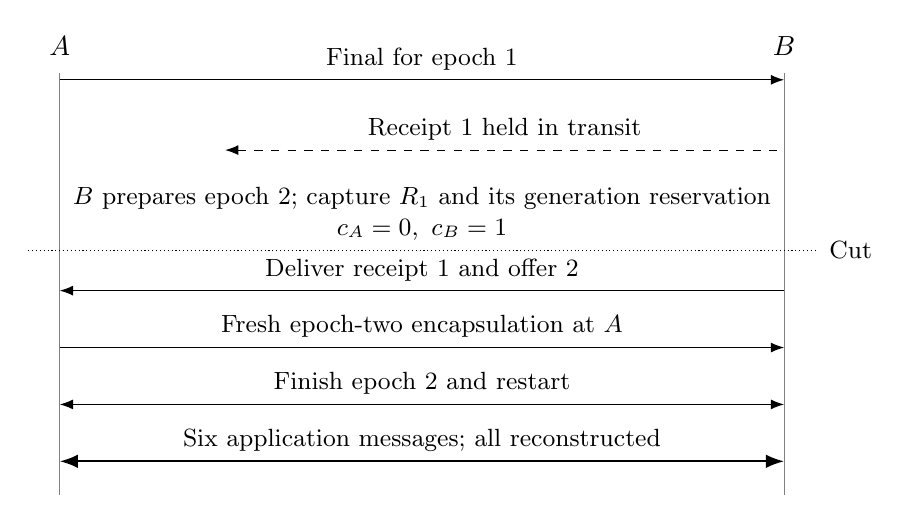
\begin{tikzpicture}[x=1cm,y=0.85cm,font=\small,>=Latex]
\node[font=\bfseries] at (0,0.5) {$A$};
\node[font=\bfseries] at (9.2,0.5) {$B$};
\draw[gray] (0,0.1)--(0,-6.2);
\draw[gray] (9.2,0.1)--(9.2,-6.2);
\draw[->] (0,0)--node[above] {Final for epoch 1}(9.2,0);
\node[align=left,anchor=west] at (9.35,-0.55) {};
\draw[<- ,dashed] (2.1,-1.05)--node[above] {Receipt 1 held in transit}(9.2,-1.05);
\node[align=center,fill=white] at (4.6,-2.0)
 {$B$ prepares epoch 2; capture $R_1$ and its generation reservation\\
  $c_A=0,\ c_B=1$};
\draw[densely dotted] (-0.4,-2.55)--(9.6,-2.55);
\node[anchor=west] at (9.65,-2.55) {Cut};
\draw[<-] (0,-3.15)--node[above] {Deliver receipt 1 and offer 2}(9.2,-3.15);
\draw[->] (0,-4.0)--node[above] {Fresh epoch-two encapsulation at $A$}(9.2,-4.0);
\draw[<->] (0,-4.85)--node[above] {Finish epoch 2 and restart}(9.2,-4.85);
\draw[<->,thick] (0,-5.7)--node[above] {Six application messages; all reconstructed}(9.2,-5.7);
\end{tikzpicture}
\caption{A retained native disclosure execution. The smaller confirmed counter
is zero at capture, while the captured reservation enables epoch-two traffic
recovery after the public exchange. The dotted Cut orders the exposure and the subsequent
fresh encapsulation; it does not refresh the earlier generation reservation.}
\label{fig:delayed-receipt}
\end{figure}

The resulting counterexample targets the proposed bound
$\min(c_A,c_B)+1$: its value is one, yet epoch-two traffic is exposed.
The protocol's asymmetric progress is legitimate. Recovery reasoning must
therefore follow the retained inputs and their descendants rather than identify
the two endpoints' confirmation counters.

% This module uses amsmath, amssymb, amsthm, and the main document's
% definition, lemma, corollary, and proof environments.
% The normalization lemma below is a new, manually proved interface result.
% The separately cited Tamarin theorem is an existing symbolic result.

\section{Reservation origins, persistent records, and recovery}
\label{sec:security-model}

An interrupted cryptographic operation can retain its random tape before it
has produced a key or a ciphertext.  Its later execution and confirmation
therefore have to be related to the original reservation.  We make this
relationship explicit at two levels: the origin of a cryptographic operation,
and the origin of a saved session-state version.  A third identifier describes
the physical image that carries that version.  This distinction lets us
account for a target record copied by another session's write, an unapplied
pending image, and a ciphertext acquired before its wrapping key.

The model is an interface model for an asynchronous protocol machine
$\mathcal P$.  The adversary schedules public messages, process loss, honest
recovery, and the disclosure operations specified below.  Application
deliveries are private to the honest applications.  Capture grants read access
to the stated assets; it does not grant an additional operation for replacing
the authoritative journal.  An implementation with adversarial rollback or
forking requires those transitions in its storage machine.  The protocol,
its cryptographic primitives, and its public outputs are parameters of the
record-normalization lemma.  Fix finite execution, record-size, and query
budgets; the wrapper's bookkeeping is polynomial in their total
representation size.

Table~\ref{tab:record-notation} summarizes the principal objects.

\begin{table}[t]
\centering
\caption{Principal objects in the record model. The three identities separate
an original random draw, an immutable session-state version and its physical
storage representation.}
\label{tab:record-notation}
\small
\begin{tabularx}{\linewidth}{@{}>{\raggedright\arraybackslash}p{.25\linewidth}X@{}}
\toprule
Notation & Meaning\\
\midrule
$o,\rho_o$ & Original invocation and its reserved random tape\\
$v,X_v$ & Immutable session-state version and its payload\\
$h$ & Physical image or pending object carrying one or more versions\\
$\kappa$ & Identity of actual key material, shared by equal keys\\
$\mathsf{res}(o)$ & Event at which the original random tape is drawn\\
$\mathsf{save}(v)$ & First retention of $v$ on the durable acquisition surface\\
$\mathcal C_t,\mathcal L_t$ & Acquired and readable original versions at prefix $t$\\
\bottomrule
\end{tabularx}
\end{table}

\subsection{Three origins and their event order}

\begin{definition}[Reservation origin]
\label{def:reservation-origin}
A reservation origin is a fresh invocation index $o$, together with
\[
  \bigl(\mathsf{kind}_o,\mathsf{owner}_o,s_o,e_o,B_o,
        \mathsf{res}(o)\bigr).
\]
Here $\mathsf{kind}_o$ distinguishes generation, encapsulation, and any other
reserved operation; $s_o,e_o$ identify its session and epoch; $B_o$ is the full
canonical binding, including the admitted policy and operation inputs; and
$\mathsf{res}(o)$ is the event at which its random tape $\rho_o$ is drawn.
Execution or exact replay of $o$ consumes the same $\rho_o$ and the same
binding.  A new draw receives a new origin even if a failed attempt's external
operation identifier is reused.
\end{definition}

The ideal source in this model draws independent tapes of the prescribed
lengths.  Explicit entropy-disclosure queries reveal designated tapes.
Independence is a distributional assumption about this source, rather than a
consequence of a later API call.  The generation and encapsulation budgets
$G,C$ count original draws, including draws in attempts that subsequently
fail.  Exact retries consume no new slot.  Independently sampled operations
retain distinct origins even if some public outputs happen to coincide.

A record version $v$ has an immutable payload $X_v$ and semantic metadata
\[
  \bigl(\mathsf{subject}(v),\mathsf{role}(v),
         \mathsf{epoch}(v),\mathsf{phase}(v)\bigr).
\]
The subject identifies the session whose state is represented, rather than
the session that most recently wrote the enclosing journal.  A version can
refer to several reservation origins and to roots or traffic state derived
from earlier origins.  Preparing a version allocates its handle.  The event
$\mathsf{Saved}(v)$ occurs when that version first enters the durable
acquisition surface, and its time is denoted $\mathsf{save}(v)$.  In particular,
an intact target in a durable pending-write intent is saved before the
corresponding image is applied.  A storage operation may have made this
transition even when its caller receives an unknown-outcome error.

A physical object $h$ has a separate creation or sealing index.  It may carry
one version, several sessions' versions, an exact earlier image, or a pending
target.  An unchanged version keeps its $v$ and $\mathsf{save}(v)$ when it is
copied, archived, applied from a pending intent, or included in a newly sealed
aggregate.  A new semantic session-state version receives a new $v$ even when
some of its fields are unchanged.  These rules distinguish the original
reservation from each session-state update that retains it.

The following transition rules specify the provenance discipline.

\begin{enumerate}
  \item \emph{Reserve and execute.}  Reserve creates $o$ at the actual draw.
  Execution uses its retained binding and tape.  Unknown-outcome
  reconciliation keeps that origin; a definite new attempt allocates another.
  \item \emph{Prepare and retain.}  Preparing $v$ fixes $X_v$ and its provenance.
  Retaining the first intact image or pending target containing $v$ emits
  $\mathsf{Saved}(v)$.  An attempt that retains no such object has no successful
  acquisition event.
  \item \emph{Copy, apply, and reseal.}  An exact copy preserves the complete
  object and its sealing origin.  Resealing creates a new sealing invocation
  and its actual new wrapper randomness, while preserving the referenced
  record versions.  Applying an existing pending target copies its retained
  bytes.
  \item \emph{Crash and resume.}  Process loss removes volatile references.
  Recovery reconstructs the retained handles and their original provenance.
  It does not turn a retained reservation into a new draw.
  \item \emph{Confirm and delete.}  Confirmation changes protocol state and may
  authorize particular host-side deletions.  Neither action changes a
  reservation's origin or removes an adversary's previously acquired copy.
\end{enumerate}

For an original reservation actually retained in $v$, causality requires
\begin{equation}
  \mathsf{res}(o)\ \leq\ \mathsf{save}(v).
  \label{eq:origin-causality}
\end{equation}
A later physical object's creation time gives an additional timestamp, not a
replacement for either side of~\eqref{eq:origin-causality}.  The interval
between drawing $\rho_o$ and first retaining it remains explicit.  The
symbolic reservation-and-save transition can represent that interval only
through a separately justified source correspondence.

\subsection{Acquisition, delayed readability, and key identity}

Wrapping-key handles resolve to identities of actual key material.  Two
session labels that designate the same key resolve to the same identity
$\kappa$.  Disclosure through either label therefore enables every acquired
wrapper protected by $\kappa$.  A rotation creates a different identity when
it creates different key material.  Signing-key identities are treated in
the same way across sessions and roles.

For each intact physical object $h$, its construction records a finite set
\[
  \mathsf{paths}(h)=\{(v,\gamma)\},
\]
where $\gamma$ is the set of wrapping-key identities on a recoverable
serialization path to $X_v$.  Multiple paths to one version are permitted.
An unprotected record has $\gamma=\varnothing$.  Nesting a wrapper adds its
key identity; aggregation unions its members' paths.  An exact ciphertext
copy keeps its paths.  Resealing decoded records reconstructs the paths under
the new wrapper and retains the same $v$ values.  Thus resealing decoded
plaintext and wrapping an old ciphertext are distinct operations.

Only intact, recoverably embedded record payloads create these paths.  A
public hash or MAC of a private record is a public computation of that record,
not a path to the record itself.  The renderer introduced below preserves
that computation and its output.  This distinction prevents a public head
query from being relabeled as a snapshot merely because its computation used
private bytes.

\begin{definition}[Record acquisition and readability]
\label{def:record-acquisition}
A successful $\mathsf{Capture}(h)$ returns the actual retained bytes of $h$
and adds an immutable copy to the adversary's archive $\mathcal A_t$.
Let $\mathcal K_t$ be the wrapping-key identities disclosed by time $t$.
Define
\begin{align}
  \mathcal C_t
    &=\{v:\exists h\in\mathcal A_t,\ \exists\gamma,\
                    (v,\gamma)\in\mathsf{paths}(h)\}, \label{eq:acquired-records}\\
  \mathcal L_t
    &=\{v:\exists h\in\mathcal A_t,\ \exists\gamma,\
          (v,\gamma)\in\mathsf{paths}(h)
          \ \wedge\ \gamma\subseteq\mathcal K_t\}.
          \label{eq:readable-records}
\end{align}
Each capture records $\mathsf{AcquireOriginal}(v,t)$ for every version in its
support, including versions already acquired through another path.
An unsuccessful request for unavailable state returns its ordinary error and
adds no acquisition.
\end{definition}

Both sets describe the specified disclosure interfaces, using provenance and
key identities.  They do not test whether the adversary has guessed a secret.
The read set can grow without another capture: if $h$ was obtained at
$t_1$ and its final missing wrapping key is disclosed at $t_2>t_1$, the
corresponding versions enter $\mathcal L_{t_2}$.  Host deletion at an
intermediate time leaves $h$ in $\mathcal A_{t_2}$.  Acquisition, by contrast,
already occurred at $t_1$.

An additional key that is explicitly recoverable from an opened record can be
included by a declared extraction rule.  In this extension, iterate
\eqref{eq:readable-records} and the declared key-extraction rules to their least
fixed point after each event.  Each rule identifies its input bytes, its
deterministic extraction algorithm, and the resulting actual key identity.
Only rules with available inputs fire.  This accounts for nested protection
without assuming that inaccessible keys have already been learned.

Signer-file capture is a separately typed disclosure.  For correspondence
with the retained symbolic theorem, it records exposure of the actual signing
key conservatively at acquisition, as does that theorem's signer-file rule.
The readability ledger can additionally record when the file's contents
become decryptable.  In particular, a wrapping-key disclosure cannot be
scoped to traffic state when the declared capture also includes the matching
signer file.

\paragraph{Constructive exposure.}
From public protocol inputs, explicit leaks, and readable record payloads, we
form a labelled replay-dependency graph.  Its edges are specified algorithms:
unseal a reservation with its matching key; regenerate a key from its original
tape; replay encapsulation on the bound offer; decapsulate a published
ciphertext; derive a root; and derive the direction-specific traffic and ACK
material.  Directly stored roots, skipped keys, and plaintext enter through
their own record fields.  For the implemented root schedule, an edge is
\[
 (R_{e-1},S_e,C_e)\longmapsto
 R_e=\mathsf{HKDF}\bigl(R_{e-1},S_e,
       D_{\rm root}\Vert H_{\rm core}(C_e),32\bigr).
\]
Closing these explicit edges over the nodes of the bounded execution yields
a computable set of message keys with replay witnesses.  It supplies positive
exposure certificates; the
confidentiality game below is the separate criterion for messages outside
the declared disclosure conditions.  Confirmation counters belong to the
public progress state and do not reset this graph.

\subsection{An original-record implementation of the copy interface}

We now isolate a property of record management that is independent of KEM
secrecy.  The following two storage machines use the same protocol machine
$\mathcal P$, random-tape source, scheduler, and cryptographic interfaces.

The \emph{literal-copy machine} materializes the immutable payload $X_v$ in
each indicated serialization position.  Its objects include current images,
pending targets, and retained historical copies.  It records the origin tags
alongside these values as private bookkeeping.

The \emph{original-record machine} keeps one immutable table entry
$\mathcal O[v]=X_v$ and represents each serialization position by a reference
to $v$.  Its wrapper maintains the physical-object directory, pending states,
adversary archive, origin tags, and key identities.  It has the following
specified interfaces.

\begin{enumerate}
  \item $\mathsf{RegisterOriginal}(v,X_v)$ is a private write by the honest
  machine.  It fixes one value at a fresh $v$.  The wrapper receives the
  handle and the provenance metadata.
  \item $\mathsf{RenderOriginal}(\theta)$ evaluates the supplied serialization
  recipe $\theta$ by dereferencing $\mathcal O$.  A recipe specifies literal
  public fields, record references, references to already rendered objects,
  and each sealing, hash, MAC, or other admitted byte-processing call.
  A fresh sealing call uses a fresh invocation index and the same prescribed
  coin distribution as the literal-copy machine.  An exact-object read or
  replay returns its cached original bytes.
  \item $\mathsf{AcquireOriginal}(v,t)$ records acquisition of that version.
  This is an event, not an assertion of decryption.  A capture's externally
  returned bytes come from the rendered object cache.
  \item $\mathsf{RevealOriginal}(v)$ returns the original payload $X_v$.
  The wrapper uses this interface for a plaintext record-opening response
  only after a captured path is enabled by the disclosed keys, and caches
  the answer for subsequent openings.
\end{enumerate}

The renderer is an explicit trusted interface in this intermediate
experiment.  It has access to the original payload table and evaluates the
stated byte operations, including operations on undisclosed payloads.
Consequently, it can produce real ciphertexts, commitment digests, and report
MACs.  This definition does not supply an algorithm for producing those bytes
from an unknown KEM-challenge tape.  It gives a precise location for the
subsequent cryptographic replacement of that interface.

The operational contract has three further requirements.
First, all publicly visible payload-dependent bytes and statuses are obtained
through the specified renderer or through $\mathcal P$'s common protocol
computation.  Memory addresses and host timing are not additional outputs of
this interface.
Second, actual byte-operation order, error responses, partial transaction
outcomes, and cryptographic-oracle calls are retained.  Caching an exact
object does not discard a native hash-validation call, observable retry, or
write attempt: such an action remains a renderer or protocol action.
Third, the reference metadata and the key-identity relation are available to
the wrapper without inspecting a selected hidden reservation's coins.
These are checkable interface conditions; none asserts the secrecy of a
record, a root, or a message.

\begin{lemma}[Alias normalization]
\label{lem:alias-normalization}
For the operations and renderer contract above, every adversary
$\mathcal A$ interacting with the literal-copy machine has an online wrapper
$\mathcal B$ interacting with the original-record machine such that their
public views have the same distribution.  Their reservation-origin ledgers,
record-save events, acquisition events, and read sets are identical after
projection onto the original handles.

The wrapper makes at most $|\mathcal L_T|$ distinct
$\mathsf{RevealOriginal}$ calls by terminal time $T$.  Repeated physical
copies, captures, and openings do not multiply this number.  The wrapper
preserves every original reservation and every fresh sealing invocation, so
it does not merge their respective cryptographic resource counts.

The statement also holds for an adversary with quantum private state and
quantum access to common public cryptographic oracles, provided the storage
interface is classical and both experiments retain the same oracle calls.
\end{lemma}

\begin{proof}
Maintain a map from every literal record occurrence to its immutable handle
$v$, and from every native object identifier to a rendered-object entry.
Couple the protocol random tapes, sealing coins, scheduler choices, and public
cryptographic oracles between the experiments.  The invariant is that
dereferencing every original-record recipe produces the corresponding
literal-copy bytes, with the same semantic provenance and physical
disposition.

For a new record, register its payload once and extend the occurrence map.
For a fresh rendering, submit the same recipe and byte-operation sequence to
$\mathsf{RenderOriginal}$.  Dereferencing gives the same inputs to every
sealing, digest, MAC, validation, and output operation.  Coupled coins and
common oracles therefore give the same bytes, statuses, and state changes.
This step retains a write that became durable before returning an error;
the caller's status does not overwrite the persistence state.

An exact copy or pending-target application copies the object reference and
its original cache entry.  Aggregation collects the corresponding original
references, and resealing evaluates the new recipe using those references.
Each operation preserves the session-record handles and their save times.
It follows by induction on the recipe constructors that
$\mathsf{paths}(h)$ is the same in both machines.  A public hash or MAC
constructor contributes its common output, rather than a spurious
record-acquisition path.

On successful capture, output the cached object bytes in both experiments
and append its immutable descriptor to the adversary archive.  For each
version in its support, emit the same acquisition event at the actual
capture time.  Preserve the ordinary error for an unavailable object.
When a matching wrapping key is disclosed, use the common key identity and
reevaluate the enabled paths in the complete adversary archive.  For an
opening response, obtain $X_v$ from $\mathsf{RevealOriginal}$ on its first
use and from the wrapper's cache thereafter.  Every such call has
$v\in\mathcal L_T$.  Shared-key aliases and later key acquisition are thus
handled without another copy of $X_v$.  The optional key-extraction extension
preserves the invariant by induction on the least-fixed-point rounds.

Host deletion removes only host references.  The adversary archive and
already returned payloads persist.  Crash and resume use the same retained
object identifiers; neither operation recreates a reservation or changes a
save event.  Ordinary protocol actions are performed by the same
$\mathcal P$ with the same results.  This completes the induction, including
adaptive choices based on any preceding response.

For quantum private state, identical classical responses and the same public
oracle transformations induce the same transformation of that state at
each interaction.  The argument introduces no measurement of a quantum
oracle query and no oracle-dependent advice.  Finally, caching each
plaintext opening by $v$ proves the query bound; reservation and fresh-seal
indices were preserved separately throughout.
\end{proof}

The lemma places multiplicity in the correct ledger.  An adversary may retain
many ciphertext aliases of one version, and those ciphertexts may have many
different public heads.  All such byte-level observations remain in the view.
The repeated payload uses one original-record opening, whereas each genuinely
fresh seal and each public hash or MAC computation keeps its own resource
accounting.

% Manuscript fragment. Requires amsmath, amssymb, amsthm.
\subsection{Explicit guarded normalization of record readability}
\label{sec:guarded-provenance}

The path and readability definitions above already account for copying and
later key disclosure. We now give their explicit guarded normalization and
an executable realization for a record-decryption specialization. Here key
derivation has fixed public edges independent of recovered plaintext. The
optional plaintext-dependent key-extraction extension remains as defined
above and is outside this specialization. The set $\Omega_{\rm src}$ below
contains reservation-source identities; it is distinct from saved record
versions and from the original-payload table $\mathcal O[v]$. Likewise,
$\mathcal E^{\rm src}_t$ projects derivability onto protected source values,
whereas $\mathcal C_t$ and $\mathcal L_t$ track acquired and readable versions.
The graph is a fixed representation of admitted retained objects, not a
replacement for the provenance transition rules or the byte renderer.


A source identifier names one original sampling operation.  An acquisition
history records what the adversary obtains, including objects obtained at
different times.  These are distinct objects of the model: a copy preserves
the former, while an additional acquisition can change the latter.

\paragraph{Immutable record graph.}
Let $\mathcal R$ be a finite set of immutable encrypted record objects.
Each $r\in\mathcal R$ has a matching decryption-key identity $\kappa(r)$,
a set of embedded child records $\operatorname{child}(r)$, and a set
$\operatorname{orig}(r)$ of protected source values in its plaintext.
Containment is acyclic.  Record identities distinguish ciphertext objects;
source identities distinguish original sampling operations.  Several
records can contain the same source.  A rewrapped record has a new record
identity and may have a new key, while retaining its source identity.
Key identities are equivalence classes of equal actual keys, rather than
names assigned independently by separate API objects.

Let $\mathcal D\subseteq\mathcal K\times\mathcal K$ be fixed public key
derivation edges.  An edge $(k,k')$ means that possession of $k$ permits
deterministic computation of $k'$.  This interface represents, for example,
derivation of an operation-wrapping key from the journal key.  In the
theorem below, these edges do not depend on plaintext recovered from records.
Write $D^*$ for their reflexive transitive closure.

Let $\Omega_{\rm src}=\bigcup_{r\in\mathcal R}\operatorname{orig}(r)$ be the
declared source domain.  At a trace prefix $t$, let $A_t\subseteq\mathcal R$ be all record objects
ever acquired by that prefix, $K_t\subseteq\mathcal K$ all directly
disclosed keys, and $\mathcal S^{\rm dir}_t\subseteq\Omega_{\rm src}$ all directly disclosed source values, represented
by their source identities.  These are cumulative sets.  The decryption-key
closure is
\[
  K_t^*=\{k':\exists k\in K_t,\ (k,k')\in D^*\}.
\]
The concrete derivation rules are
\[
 \frac{k\quad(k,k')\in\mathcal D}{k'},\qquad
 \frac{r\quad\kappa(r)}{c}\ (c\in\operatorname{child}(r)),\qquad
 \frac{r\quad\kappa(r)}{o}\ (o\in\operatorname{orig}(r)).
\]
Their least closure starts from $A_t,K_t,\mathcal S^{\rm dir}_t$.  A fact $o$ in the source
sort means that the protected value of source $o$ is derivable; it does
not mean that a public identifier has become known.  The source projection
of this closure is denoted $\mathcal E^{\rm src}_t$.

\paragraph{Guarded routes.}
For every path $p=(r_0,\ldots,r_\ell)$ in the containment graph ending
at a record with $o\in\operatorname{orig}(r_\ell)$, define
\[
 g(p)=\{\kappa(r_0),\ldots,\kappa(r_\ell)\}.
\]
The normalized table contains a route $(r_0,g(p),o,p)$ for every such
path.  Its exposure expression is
\[
 \widehat{\mathcal E}^{\rm src}_t=\mathcal S^{\rm dir}_t\ \cup\
 \{o:\exists(r,g,o,p),\ r\in A_t\ \land\ g\subseteq K_t^*\}.
 \tag{GP}
\]
Alternative records and paths are disjoined, while all keys on one path
are conjoined.  Equal key identities occur only once in the guard set.

\begin{theorem}[Exact guarded normalization]
\label{thm:guarded-normalization}
For every finite record graph and derivation interface above, and every
acquisition prefix $(A_t,K_t,\mathcal S^{\rm dir}_t)$, the concrete and normalized exposure
sets agree: $\mathcal E^{\rm src}_t=\widehat{\mathcal E}^{\rm src}_t$.  The equality applies to all prefixes of
an adaptively chosen history.
\end{theorem}
\begin{proof}
Key derivations depend only on disclosed keys and the fixed relation
$\mathcal D$, so their least closure is exactly $K_t^*$.
For the forward inclusion, take a source $o\in \mathcal E^{\rm src}_t$.
If it was directly disclosed then $o\in \mathcal S^{\rm dir}_t$.
Otherwise its first derivation decrypts a record $r_\ell$ with the
matching key.  If that record was not acquired directly, its first
availability follows by decrypting a parent.  Follow these first
derivations backwards.  The finite acyclic record graph makes this
process terminate at an acquired record $r_0$.  Every intervening key
lies in $K_t^*$, yielding a route satisfying (GP).
For the reverse inclusion, take a satisfied route.  Starting with its
acquired first record, successively decrypt along the path.  Every
required key is in $K_t^*$, so each child and finally $o$ is in the
concrete least closure.  Direct disclosures are in that closure by
definition.  Both inclusions hold for each fixed prefix; no independence
or advance choice of the acquisition schedule was used.
\end{proof}

\paragraph{Efficient evaluation.}
Equation (GP) is a declarative normal form: a compressed record DAG can
have exponentially many paths.  An efficient leakage evaluator instead
computes the iterative decryption and key-derivation fixed point, without
enumerating those paths.  Let $N$ be the total number of record, key and
source atoms, and let $M$ count rule and payload incidences.  There are at
most $N$ strict-growth rounds; repeated rule scans therefore take
$O(N(N+M))$ time and $O(N+M)$ space under standard indexed set and
dictionary representations, with source-dictionary operations included
in this accounting.  The finite checker materializes the route table only
for its declared small fixtures, to compare that normal form against the
forward evaluator.

\begin{corollary}[Copies, deletion and late disclosure]
\label{cor:guarded-history}
Exposure is monotone under additional acquisitions, direct disclosures
and key disclosures.  Copying or rewrapping a source adds routes to the
same source identity.  Local deletion of a record previously acquired
does not remove its routes from adversarial knowledge.  In particular,
a later matching-key disclosure can expose a source in a ciphertext
acquired before that disclosure and deleted locally in the meantime.
\end{corollary}
\begin{proof}
The cumulative sets and their key closure only grow, and every predicate
in (GP) is positive.  A source-preserving copy changes a route's record
identity or key guards but not its terminal source.  Local deletion
restricts future acquisition from that local store; it removes no member
of $A_t$ and therefore cannot invalidate a satisfied route.
\end{proof}

\paragraph{Interface significance.}
The theorem gives an exact finite normalization of the chosen
record-decryption semantics.  It supports a precise original-operation
leakage oracle: a query for source $o$ can be evaluated against the
complete acquisition history, with a path and its key guards as a witness.
The cryptographic transition from native ciphertexts and public
commitments to this interface has a separate simulation obligation.
The derivation rules do not model guessing, cryptanalysis, timing leakage
or a quantum decryption oracle.  Accordingly, absence from $\mathcal E^{\rm src}_t$ is
recorded as non-derivability by these rules; message indistinguishability
outside an exposure set is supplied by a security theorem for the
surrounding protocol.

\paragraph{Native shape and finite checks.}
At the fixed research source, operation reservations are encrypted under
a wrapping key derived from the journal key, and tokens are retained
within encrypted durable images or pending targets.  The corresponding
route therefore includes the image key and the token key, with their
actual derivation edge.  A fresh aggregate image can preserve an older
token and its original source.  Public image-head digests are distinct
observations from the record objects needed by the decryption rules.
The executable supplement independently evaluates iterative decryption
and guarded-route normalization, exhausts all acquisition/key/direct-source
subsets for its declared finite graphs, and checks histories with late
key disclosure and local deletion.  Its counts and source hash are in
the accompanying machine-readable result; those checks validate the
implemented finite model and supplement the general proof above.

% Standalone manuscript fragment; no preamble.
% Requires proposition and proof environments (e.g. amsthm).
\paragraph{Why exposure must retain conjunctive guards.}
The following elementary separation explains the conjunction in (GP).

\begin{proposition}[Acquisition exposure is not additive]
\label{prop:acquisition-nonadditivity}
Let $r$ be a retained-record atom, $k$ a wrapping-key atom, and $s$ a
protected-seed atom associated with an origin identifier $o$.
For $A\subseteq\{r,k\}$, let $\operatorname{Cl}(A)$ be the least set
containing $A$ and closed under the rule
\[
  \{r,k\}\;\Longrightarrow\;s.
\]
There are no other rules in this fragment.  Define the exposed-origin set by
\[
  E(A)=\{\,o : s\in\operatorname{Cl}(A)\,\}.
\]
There is no fixed function
$f:\{r,k\}\longrightarrow\mathcal{P}(\{o\})$ satisfying
\[
  E(A)=\bigcup_{x\in A} f(x)
  \qquad\text{for every }A\subseteq\{r,k\}.
\]
\end{proposition}

\begin{proof}
The closure rule gives
\[
  E(\{r\})=E(\{k\})=\varnothing,
  \qquad
  E(\{r,k\})=\{o\}.
\]
Exactness for the two singleton acquisitions forces
$f(r)=f(k)=\varnothing$.  Their union is then empty for the joint
acquisition, contradicting $E(\{r,k\})=\{o\}$.
\end{proof}

\paragraph{Meaning of exposure.}
Membership of an origin $o$ in $E(A)$ records derivability of its
protected seed under the specified closure rules; the identifier itself
may be public. Computational estimation is measured separately by success
probability. A one-time-pad illustration makes the dependence on joint
observations explicit: let $S,W$ be independent uniform $\lambda$-bit strings and
$C=S\mathbin{\oplus}W$, with no additional observation depending on $S$ or
$W$.  Then
\[
  H(S\mid C)=H(S\mid W)=\lambda,
  \qquad H(S\mid C,W)=0.
\]
From either observation alone, any estimator of $S$ succeeds with
probability at most $2^{-\lambda}$; from both, $S=C\mathbin{\oplus}W$
recovers it exactly. The XOR construction serves here as an
information-theoretic illustration of acquisition; the protocol's record
encryption is handled by its cryptographic record interface.

\paragraph{Consequence for provenance routes.}
A source label and an exposure decision serve different purposes.  Copying
a retained record preserves the source label, while subsequent acquisition
of a matching key may change exposure.  A guarded-route representation
retains this distinction: alternative acquired records supply alternative
routes to the same source, and every route retains the conjunction of its
required keys.  Exposure is therefore evaluated from the joint acquisition
and key-derivation history. The separation applies specifically to an
exact exposure representation formed by the union of fixed per-object
labels.


\subsection{A recovery experiment with acquisition-based eligibility}

\begin{definition}[Fixed-target recovery experiment]
\label{def:recovery-game}
Fix a protocol profile $\mathcal P$ and finite execution budgets, together with
a designated session $s$, recovery cut $c$, target epoch $e$, and candidate
generation and encapsulation reservation handles $g_e,a_e$.  Handles may be
named by original invocation slots before those invocations occur; a missing
invocation will fail the reservation-event test below.  Public
protocol messages may be delayed, duplicated, reordered, or replaced.
The adversary can capture the declared retained objects, reveal wrapping
keys, reveal actual signing keys or signer files, and reveal designated
reservation tapes.  The cut exposes the selected wrapping keys; preceding
roots may already be public or disclosed by the stated prior captures.
These disclosures have their exact scope in the event ledger.

For one fresh logical application send, the adversary supplies equal-length
messages $(m_0,m_1)$.  The challenger samples $b\leftarrow\{0,1\}$ and runs
the ordinary sending transition on $m_b$.  Rejection or an unknown outcome
keeps its ordinary protocol behavior.  A retained accepted send is identified
by $(s,e,d,j)$, including direction $d$ and the epoch-scoped logical index $j$;
exact retries reuse its original ciphertext.  The challenge is valid only
when that logical send is accepted in the designated epoch.  Subsequent
protocol actions and disclosures continue until the adversary outputs $b'$.
\end{definition}

Write $\iota_A,\iota_B$ for the two actual signing-key identities configured
for the target session.  The predicate
$\mathsf{ReservedFor}(s,e,g_e,a_e)$ checks the occurrence of the named honest
generation and encapsulation reservation events in the target epoch's local
durable plans, with their target session and roles.  It checks event metadata,
without asserting that their outputs form the accepted target exchange.
Eligibility uses the following event conditions over the complete execution:
\begin{align}
 \mathsf{Eligible}_{s,e,c}(\tau)\ \Longleftrightarrow\quad&
 \mathsf{ValidTarget}(\tau)
 \ \wedge\ \mathsf{ReservedFor}(s,e,g_e,a_e)
 \nonumber\\[-1mm]
 &{}\wedge\ c<\mathsf{res}(g_e)
          \ \wedge\ c<\mathsf{res}(a_e)
 \nonumber\\
 &{}\wedge\ \iota_A,\iota_B
                  \notin\mathsf{IdentityExposed}(\tau)
 \nonumber\\
 &{}\wedge\ \mathsf{EntropyExposed}(s,e;\tau)=\varnothing
 \nonumber\\
 &{}\wedge\ \nexists v\in\mathcal C_T:
       \mathsf{subject}(v)=s\ \wedge\ c<\mathsf{save}(v).
 \label{eq:eligibility}
\end{align}
Here $\mathsf{EntropyExposed}(s,e;\tau)$ records the target epoch's designated
entropy disclosures.  The separate event $\mathsf{Attr}$ states that these
named reservation events form the accepted target's unique usable
generation/encapsulation pair, with an adapter-computable association to the
original slots.  In particular, it connects the generation public key, the
encapsulation input, the authenticated response, and the target's subsequent
key schedule.  This matching is a
source/authentication obligation, rather than an additional eligibility
filter: a failure of $\mathsf{Attr}$ can occur while
$\mathsf{Eligible}_{s,e,c}$ holds and is charged in the computational
accounting.

The final line of~\eqref{eq:eligibility} concerns every saved version of session
$s$, across its roles and epochs.  It uses acquisition
$\mathcal C_T$, including protected bytes, rather than delayed readability
$\mathcal L_T$.  Other epochs' entropy disclosures retain their ordinary
behavior.  Both peers' confirmation is not an additional send prerequisite.

Define the unconditional centered advantage by
\begin{equation}
 \mathsf{Adv}^{\rm rec}_{\mathcal P}(\mathcal A)
   =
 \left|
   \mathbb E\!\left[
    \mathbf 1_{\mathsf{Eligible}_{s,e,c}(\tau)}
                       (-1)^{b\oplus b'}\right]
 \right|.
 \label{eq:recovery-score}
\end{equation}
Invalid or ineligible executions contribute zero.  This definition retains
failures and adaptive disclosures in the probability space and avoids
conditioning a reduction on an uncontrolled eligibility probability.
If every execution with $\mathsf{Eligible}_{s,e,c}=0$ is completed by an
independent fair guess, the conventional advantage over one half is
\[
 \mathsf{Adv}_{\rm msg}
   =\left|\Pr[\text{completed guess is correct}]-\tfrac12\right|
   =\tfrac12\,\mathsf{Adv}^{\rm rec}_{\mathcal P}(\mathcal A).
\]
The computational accounting uses this latter convention.

The adaptive version retains one application challenge and permits the
candidate selector to choose its coordinates and reservation-event handles
from the observed interaction, rather than fixing them at setup.  Eligibility
requires those coordinates to identify the challenge's accepted logical send;
selection never transfers its test bit to another send.  Eligibility
and the usable-pair attribution are evaluated on that experiment's complete
history.  An origin-pair reduction fixes a slot pair in $[G]\times[C]$ and
scores the event that the final selector attributes the target to that pair.
The selector and disclosure predicates are recomputed in each comparison
world.  No independence between that selection and the transcript is imposed.

The record restriction in~\eqref{eq:eligibility} is the one used by the
retained multi-epoch symbolic theorem: its \textsf{Snapshot} action outputs
a protected record, while \textsf{Cut} separately releases the wrapping keys.
The theorem establishes symbolic plaintext secrecy with both original
reservations after the cut, key-scoped identity exclusions, the target
entropy exclusion, and the stated post-cut saved-record acquisition
exclusion~\cite{qperiaptSymbolic2026}.  Its joint replay verifies the main
lemma and all 24 reusable dependencies.  Equation~\eqref{eq:recovery-score}
specifies the computational message experiment to which the cryptographic
modules are to be connected; the alias lemma establishes its record-interface
normalization.

\begin{corollary}[Safe stopping at a forbidden acquisition]
\label{cor:target-acquisition-stop}
Consider the fixed-target experiment of
Definition~\ref{def:recovery-game}.  Suppose an actual successful capture
contains a target-session version $v$ with $c<\mathsf{save}(v)$, identified
by the original-record metadata.  For any terminal bit $D$, replacing the
remainder of that execution by output zero leaves
\[
   \Pr[\mathsf{Eligible}_{s,e,c}(\tau)\wedge D=1]
\]
unchanged.  Replacing its terminal score by zero also leaves the expectation
inside~\eqref{eq:recovery-score} unchanged.

In particular, if a captured target-session version retains the selected
reservation $o\in\{g_e,a_e\}$, then
$c<\mathsf{res}(o)$ and~\eqref{eq:origin-causality} establish this stopping
condition.  The wrapping key may be obtained before or after the capture.
\end{corollary}

\begin{proof}
The successful capture inserts $v$ into $\mathcal C_t$ immediately.
Its save time and subject are immutable, and acquisition remains recorded
after host deletion, resealing, confirmation, or process loss.  Thus the
last conjunct of~\eqref{eq:eligibility} is false for every continuation.
Each such continuation already contributes zero to both quantities.
On executions that never reach this condition, the experiment is unchanged.
The final assertion follows from
$c<\mathsf{res}(o)\leq\mathsf{save}(v)$.
\end{proof}

The stopping test uses the successful acquisition event and its record
metadata; it can run before the response's private bytes are serialized by
a challenge adapter.  It is not an SDK rejection of the capture.  A public
digest, an unrelated record, or an unsuccessful capture keeps its real
behavior.  In particular, difficulty computing a permitted digest or report
MAC does not trigger this corollary.
For adaptive target selection, stopping is applied to the corresponding
fixed-candidate event in the reduction.  One possible candidate becoming
ineligible does not justify terminating a game that can still select a
different eligible target.

Two short executions illustrate why both kinds of origin are necessary.
If $v$ was saved before $c$ and a sibling write reseals it after $c$, the
acquisition still refers to the original pre-cut $v$.  The new global image
time alone does not falsify the final conjunct of~\eqref{eq:eligibility}.
If instead $v$ was saved after $c$, a later write attributed to a sibling
does not change its subject or make its capture eligible.  Likewise, a
pre-cut generation reservation retained through a delayed receipt remains
pre-cut when its KEM computation completes later.  Its reservation condition,
rather than the slower endpoint's confirmed counter, determines that case.

\subsection{Connection to the cryptographic argument}

The normalization theorem fixes the original objects whose bytes, acquisition,
and key identities the reduction must represent. The next section gives
constructive image/intent and report interfaces for a selected KEM operation
whose public outputs are available while its original random tape is opaque.
Their algorithms preserve original-object caches, public commitments, exact
retries, and actual durable outcomes. The fixed-target stopping rule above
extends to an adaptive provenance certificate in
Lemma~\ref{lem:adaptive-origin-stop}.

Usable attribution is computed from available semantic metadata. Original
generation and encapsulation slots belong to a fixed lifetime budget
$[G]\times[C]$: a fresh draw receives a new slot, while copies retain their
source. Each candidate induces its own protected records and report-key
closure. Proposition~\ref{prop:native-local-accounting} decomposes the score
in the native experiment before comparing those local continuations. It
retains both unattributable eligible executions and permitted key projections
as explicit native-game terms.

The computational composition evaluates accepted operations, eligibility, and
all public outputs anew in each comparison world. Exact component repeats
retain one response and one correctness event. The native constructor map in
Section~\ref{sec:native-correspondence} identifies the storage operations used
by these interfaces; Section~\ref{sec:discussion} specifies the joint root and
message continuation to which their bounds connect.

\section{Mechanized recovery and separating executions}
\label{sec:established}

\subsection{The multi-epoch symbolic theorem}

The checked symbolic model includes inherited roots, alternating proposers,
asymmetric confirmation, initial traffic, and unbounded epochs. Signing and
wrapping keys may be shared across their modeled uses. Its \textsf{Cut} event
exposes the selected wrapping keys; exposure of other epochs' entropy is
represented separately. We state the main theorem in terms of its recorded
events, preserving its original target and disclosure predicates.

Let $\tau$ be a trace of that model. Write
$\mathsf{SessionKeys}(s,a,b)$ for the actual identity keys associated with session
$s$, $\mathsf{KeyReserved}(s,e,P)$ and $\mathsf{EncapReserved}(s,e,Q)$ for the
target reservations, and $\mathsf{Message}(s,e,r,k,m)$ for an application-message
event. Define $\mathsf{AcquiredAfterSave}_c(s)$ to hold when there exist a role,
an epoch, a revision, and matching \textsf{Saved}/\textsf{Snapshot} events for
session $s$, with the \emph{save} event strictly after $c$. The matching record's
session projection is the relevant saved object.

\begin{theorem}[Checked multi-epoch symbolic secrecy]
\label{thm:symbolic}
Suppose $\tau$ contains the corresponding \textsf{SessionKeys}, \textsf{Cut}
at $c$, target reservation events at $g$ and $h$, and
$\mathsf{Message}(s,e,r,k,m)$. If
\[
 c<g,\qquad c<h,
\]
neither actual target identity key is disclosed anywhere in $\tau$, no reserved
entropy of target epoch $e$ is disclosed, and
$\mathsf{AcquiredAfterSave}_c(s)$ is false, then $\tau$ contains no adversarial
knowledge event $\mathsf K(m)$.
\end{theorem}

The theorem was checked with all 24 reusable dependencies in one Tamarin
process. An independent replay produced a byte-identical proof certificate.
Appendix~\ref{app:artifacts} identifies the exact query, source, toolchain,
replay receipt and complete auxiliary-query inventory.

The theorem uses the modeled cryptographic constructors and record interface.
Its key scope follows actual identity ownership: a shared signer exposed through
another session is still a disclosure of that target key. Likewise, a retained
target projection saved after Cut remains subject to the acquisition condition
when a sibling write carries it into a later aggregate image.

\subsection{Executability and the freshness boundary}

A finite two-round construction exercises the operational rules with an exposed
ancestor root and satisfies the complete original positive existential formula.
A separate source-derived evaluator checks its rule instances and global
quantifiers. This provides a concrete execution for the modeled recovery
premises.

The delayed-receipt construction instead contains a pre-Cut epoch-two
generation reservation and a post-Cut encapsulation. It derives the target
payload while satisfying the remaining main-theorem antecedents. Its point
audit identifies $c<g$ as the sole false antecedent. Seven countertraces are
rejected by the witness checker. Together, the positive and separating traces
connect the recovery condition to executable schedules.

\subsection{Native reservation disclosure}

The native experiment stops a child process after committing a reservation,
kills and reaps it, reopens the journal, and inspects the retained phase.
It exercises two distinct boundaries:
\begin{itemize}
\item a 277-byte key-generation token, before key computation or offer publication;
\item a 245-byte encapsulation token, after offer authentication and before
encapsulation computation or response publication.
\end{itemize}
The predictor obtains the previous root, journal identity, wrapping key and
captured token. Thereafter it uses the public policy configuration and later
authenticated control wires. Its prediction interface has no journal or
filesystem input, and the experiment withholds signer files and future private
owners. A wrong wrapping key is rejected.

For each cut, both honest peers complete the rekey and reopen their journals.
The driver then creates fresh 128-byte application payloads, sends three in each
direction, and checks honest delivery. Independently reconstructed traffic
owners authenticate and decrypt all six intercepted frames. The two cuts
therefore yield twelve actual post-restart plaintext recoveries. The
delayed-receipt extension repeats the six-message check at epoch two using one
responder snapshot.

\begin{proposition}[Execution-time and counter-based separation]
\label{prop:counter-separation}
In the native executions, computing a KEM after restart, completing
the target epoch, and subsequently reopening the journal do not make a
previously disclosed reservation an independent secret contribution.
Moreover, $\min(c_A,c_B)+1$ is not a universal upper bound on exposed epochs.
\end{proposition}
\begin{proof}
At both process-cut boundaries the captured reservation reconstructs the later
honest KEM result exactly. Equations~\eqref{eq:root}--\eqref{eq:traffic} then
reconstruct traffic keys from the captured predecessor root and public wires;
authenticated decryption verifies the six corresponding plaintexts after
completion and restart. In the delayed-receipt execution,
$(c_A,c_B)=(0,1)$ at capture and six epoch-two plaintexts are recovered.
Thus the proposed counter bound equals one while an exposed epoch equals two.
\end{proof}

\subsection{An aggregate write preserves the target origin}

A separate two-session native execution changes a sibling session and writes a
new aggregate image. It checks exact equality of the retained target record,
reopens and retries the original operation, and decrypts six subsequent target
messages in each build profile. The new global revision and outer encryption
nonce coexist with the old target reservation. This execution instantiates the
alias/provenance distinction in the record model.

The native executions isolate the reservation and acquisition conditions
used in Theorem~\ref{thm:symbolic}. Section~\ref{sec:computation} gives the
record simulations and common-experiment accounting for the corresponding
computational interfaces.


\section{Executable reference corpora and comparison design}
\label{sec:evaluation}

The executable references provide reproducible observations of communication
and exposure. The pinned SPQR source is
\texttt{f2589fef855c10f39d72634dab3d14654dd410bf}. Seven schedules each contain
2,048 sends: alternating, loss, reordering, duplication, 9:1 asymmetry,
offline-then-exchange, and one-way traffic. Six capture points for each endpoint
produce 84 passive snapshot cases. The whole-KEM control runs those schedules
at local-send intervals 1, 32 and 64, producing 252 corresponding cases.
Together these are 28 configuration/schedule combinations and 336 snapshots.
The explicitly modified 64-byte SPQR variant has its own source identity.

\subsection{Observed derivation and communication}

The snapshot predictor receives one endpoint's serialized state and the full
public transcript, including packets lost before peer delivery. A separate
harness compares every derived key with the actual sender's key. Public
deterministic seeds are test fixtures; the measurement establishes causal key
derivation through the declared predictor interface. The output label
\texttt{not\_derived} denotes that predictor's result. It is separate from the
security predicate of a computational experiment.

Table~\ref{tab:reference} reproduces the retained alternating-schedule
observations. The snapshot is taken at $A$ immediately after its first send,
leaving 2,047 future sends. The pending KEM key accounts for 87 of the 172
derived keys in the pinned 32-byte SPQR case, demonstrating why the currently
emitted chain epoch alone does not describe exposure.

\begin{table}[t]
\centering
\small
\begin{tabular}{@{}lrrrr@{}}
\toprule
Component/profile & Mean bytes/send & Peak frame & Epochs $A/B$ & Derived keys\\
\midrule
Pinned SPQR, 32 B & 32.150 & 37 & 24/23 & 172\\
SPQR variant, 64 B & 58.971 & 69 & 46/45 & 88\\
Whole KEM, interval 1 & 819.658 & 1,225 & 683/683 & 4\\
Whole KEM, interval 32 & 44.047 & 1,223 & 32/32 & 66\\
Whole KEM, interval 64 & 25.023 & 1,223 & 16/16 & 130\\
\bottomrule
\end{tabular}
\caption{Retained component-level alternating workload. Byte counts are the
component wire contribution; epoch counts are each component's root/output
observations. The constructions have different authentication and retention
graphs. Outer application AEAD, transport, durable storage and energy are
outside these measurements.}
\label{tab:reference}
\end{table}

The one-way schedule produces no fresh PQ epoch in these references and the
predictor derives every post-snapshot key. The whole-KEM active-control
experiment addresses a different property: one initial endpoint-state capture
allows two attacker forks to replace subsequent exchanges while honest
confirmed epochs increase. All 1,536 sender keys across three 512-send profiles
match the attacker-derived keys. This supplies a concrete distinction between
fresh KEM execution and authenticated recovery when the ongoing authentication
authority is itself derived from captured session state.

\subsection{Aligning the Continuity experiment}

A matched experiment must give each construction the same application and
control-message opportunities and the same loss, reorder and duplication
schedule. Authentication capabilities are recorded explicitly: the whole-KEM
control uses session-state authentication, whereas Continuity controls use
the separately modeled device signing authority. Serialized volatile state,
retained reservations and actual durable journal images are distinct disclosure
objects.

The planned Continuity comparison records, for each exposure case, the original
generation and encapsulation reservation identifiers, the retained record
projection, acquired wrapping-key identifiers, endpoint phase/counter state,
public-wire availability and the actually reconstructed message set.
Communication records include total bytes and largest frame. Persistence
records include durable writes, restart/retry work and retained-state size.
Each timing denominator covers its declared operation interval and names the
compiler profile, primitive backend, host and sample unit.

The principal ablations hold the underlying reservation fixed while changing
its execution time, delay a receipt, copy a target through a sibling aggregate
write, and compare origin-preserving labels with labels based on the last image
write. These ablations test the mechanisms isolated by the theorem and
separating executions. Their comparison will explain both exposure and cost
under each matched workload.

\section{Computational accounting and the common experiment}
\label{sec:computation}

The origin model provides the accounting boundary for a computational
experiment. Each original generation or encapsulation invocation receives a
slot when its entropy is reserved, including attempts that later fail.
Replaying or copying that reservation retains its slot. Fix public lifetime
budgets $G,C\geq1$ and write $J=[G]\times[C]$. Unused slots remain unused.
These proof-resource budgets differ from a bound on the number of records
resident at one time.

\subsection{A selected-target experiment}

Let $V$ be the virtual original-record experiment with the real KEM component.
The adversary chooses its target after its observed interaction. Eligibility
$E$ retains the selected recovery conditions: both original target reservations
follow Cut, the actual target signing keys and target-epoch entropy remain
unexposed, and no selected-session record saved after Cut is acquired.
The experiment follows allowed asynchronous control and application transitions,
including sending after the local FinalReady transition.

Let $\mathsf{Attr}$ mean that the selected target has a unique usable pair of
original slots, and let $I\in J$ denote that pair. The mapping and every event
used by the reduction must be computable from the adapter's known semantic
state and observations. Let
\[
 \eta\ \geq\ \Pr_V[E\wedge\neg\mathsf{Attr}].
\]
For $j\in J$, define $V_j$ as the full experiment with the adapter's random
component override at pair $j$. Its transcript, eligibility and target choice
are recomputed in that world. The remaining protocol and oracle calls use
the same common interfaces.

The application test bit is sampled by the surrounding simulator. Write
$S=+1$ for a correct guess and $S=-1$ otherwise; invalid tests contribute zero
through $E$. Every $E=0$ execution is completed by an independent fair guess. Thus the
usual message-guessing advantage is
$\tfrac12|\mathbb E[E S]|$.
The simulator can evaluate this score without observing the hidden bit of its
component KEM challenger.

\subsection{Centered-score composition}

For each $j$, put $E_j=E\wedge\mathsf{Attr}\wedge(I=j)$.
Suppose the fixed-pair component adapter gives, for $\sigma\in\{+1,-1\}$,
\begin{equation}
\left|\Pr_V[E_j\wedge S=\sigma]
      -\Pr_{V_j}[E_j\wedge S=\sigma]\right|
 \leq a_j^\sigma+\delta_j,                         \label{eq:component-hop}
\end{equation}
where $a_j^\sigma$ is the advantage of the actual derived component
distinguisher and $\delta_j$ is the corresponding correctness term.
The distinguisher includes target selection and all relevant oracle queries.
Define
\[
 b_j=\mathbb E_{V_j}[E_jS].
\]
Finally, let $\epsilon_{\rm rec}$ bound the binary distinguishing gap between
the native and virtual experiments for their efficiently evaluable
positive-score and negative-score events. This is the concrete record-interface
connection, including public outputs and accepted operation histories.

\begin{proposition}[Adaptive origin-pair accounting]
\label{prop:adaptive-accounting}
Under these stated interface and fixed-pair bounds, the native application's
guessing advantage satisfies
\begin{equation}
\operatorname{Adv}_{\rm msg}
 \leq \min\left\{\frac12,\
 \epsilon_{\rm rec}+\frac12
 \left(\eta+\sum_{j\in J}|b_j|
       +\sum_{j\in J}(a_j^{+}+a_j^{-}+2\delta_j)\right)\right\}.
\label{eq:accounting}
\end{equation}
\end{proposition}
\begin{proof}
In the single experiment $V$, the attributed events $E_j$ are disjoint.
Decomposing its score yields
\[
 \mathbb E_V[ES]
 =\mathbb E_V[ES\,\mathbf1_{\neg\mathsf{Attr}}]
   +\sum_{j\in J}\mathbb E_V[E_jS].
\]
The first term has magnitude at most $\eta$. Each attributed expectation is the
positive-event probability minus the negative-event probability. Applying
\eqref{eq:component-hop} to those two events and then the triangle inequality
bounds its distance from $b_j$ by
$a_j^++a_j^-+2\delta_j$. Summing gives the virtual score bound.
The two native/virtual binary-event comparisons contribute at most
$2\epsilon_{\rm rec}$ to the score difference. Dividing by two and using the
maximum bit-guessing advantage proves \eqref{eq:accounting}.
\end{proof}

The selector may depend adaptively on its entire observed transcript.
The absolute values in $\sum_j|b_j|$ retain each override world's own target
selection. In particular, the override probabilities are not normalized as
though they belonged to one common ideal distribution. The score decomposition
also retains failed and ineligible executions in the experiment, avoiding an
uncontrolled division by the probability of eligibility.

Uniform bounds $|b_j|\leq\beta$, $a_j^\sigma\leq a$, and
$\delta_j\leq\delta$ give
\[
 \operatorname{Adv}_{\rm msg}
 \leq \min\left\{\frac12,\
 \epsilon_{\rm rec}+\frac{\eta}{2}
       +\frac{GC}{2}(\beta+2a+2\delta)\right\}.
\]
Alias proliferation changes the record inventory while preserving the original
slot count. This is the point at which origin-preserving record accounting
enters the reduction.

\subsection{The joint root and message interface}

The root derivation in \eqref{eq:root} begins with
\[
 p_e=\operatorname{HMAC}_{R_{e-1}}(S_e).
\]
After disclosure of $R_{e-1}$, the secret is in HMAC's message input.
The applicable extractor/swap-PRF condition therefore concerns that input
distribution; ordinary PRF security for an unknown HMAC key is a different
premise~\cite{hmacswap2023,rfc5869}. The retained computational notes instantiate
the actual input lengths and domains, treat shared root uses and aliases,
and state the corresponding quantum-oracle accounting.

The quantities in \eqref{eq:accounting} organize the next two cryptographic
connections. To bound $\epsilon_{\rm rec}$ and $\eta$, the concrete adapter must
simulate protected pending writes, public commitments, replay results, report
keys and permitted acquisition using original operation handles, while matching
the source's accepted histories. To bound each $b_j$, the random-component
world must jointly generate root extraction, confirmation tags, traffic,
acknowledgements and successor epochs. Replacing a contribution before producing
its dependent controls keeps those descendants consistent.

The current record-interface lemma and source-derived event definitions isolate
the provenance part of the first connection. The existing root-extraction, shared-HMAC,
KEM-adapter and adaptive-target modules supply its cryptographic interfaces
and the second connection's component statements. Equation~\eqref{eq:accounting}
is a proved accounting proposition with these explicit inputs; completing the
common experiment requires concrete bounds for those inputs.


\bibliographystyle{alpha}
\bibliography{references}
\clearpage
\appendix
\section{Source and evidence map}
\label{app:artifacts}

The source snapshot for this manuscript's established protocol and experiment
records is commit
\texttt{228c944fc476e3e57d6c08063cacb19bca5b360e}
of \href{https://github.com/billlza/q-periapt}{\texttt{billlza/q-periapt}}.
Each retained execution keeps its original source and tool identity.
The local record model and accounting proofs in this manuscript are mathematical
arguments; the following entries identify the independently recorded
mechanization and native observations.

\begin{longtable}{@{}>{\raggedright\arraybackslash}p{0.25\linewidth}>{\raggedright\arraybackslash}p{0.69\linewidth}@{}}
\toprule
Result & Reproduction source\\
\midrule
\endhead
Joint symbolic replay &
\href{https://github.com/billlza/q-periapt/tree/228c944fc476e3e57d6c08063cacb19bca5b360e/research/sdk-alpha1/evidence/20261104-multi-epoch-replay}{20261104-multi-epoch-replay}.
The original archive is \texttt{CAPTURE.zip}; the checked certificate member is
\texttt{replay-01/01-baseline-replay.proof.spthy}.\\[5pt]
Positive two-round trace &
\href{https://github.com/billlza/q-periapt/tree/228c944fc476e3e57d6c08063cacb19bca5b360e/research/sdk-alpha1/evidence/20261105-two-round-ground-trace}{20261105-two-round-ground-trace}.\\[5pt]
Delayed-receipt ground trace &
\href{https://github.com/billlza/q-periapt/tree/228c944fc476e3e57d6c08063cacb19bca5b360e/research/sdk-alpha1/evidence/20261105-delayed-receipt-ground-trace}{20261105-delayed-receipt-ground-trace}.\\[5pt]
Native reservation disclosure &
\href{https://github.com/billlza/q-periapt/blob/228c944fc476e3e57d6c08063cacb19bca5b360e/research/continuity-identity-candidate/RESERVATION_DISCLOSURE.md}{RESERVATION\_DISCLOSURE.md}
and \path{src/durable/messages/tests/reservation_disclosure.rs}
in the identity candidate.\\[5pt]
Aggregate-copy execution &
\href{https://github.com/billlza/q-periapt/tree/228c944fc476e3e57d6c08063cacb19bca5b360e/research/sdk-alpha1/evidence/20261105-aggregate-reservation-copy}{20261105-aggregate-reservation-copy}.\\[5pt]
Root, traffic and phase mapping &
\href{https://github.com/billlza/q-periapt/blob/228c944fc476e3e57d6c08063cacb19bca5b360e/docs/continuity/RECOVERY_DEPENDENCIES_V1.md}{RECOVERY\_DEPENDENCIES\_V1.md};
native \texttt{rekey/response.rs} and \texttt{rekey/completion.rs}.\\[5pt]
SPQR snapshot corpus &
\href{https://github.com/billlza/q-periapt/tree/228c944fc476e3e57d6c08063cacb19bca5b360e/research/continuity-spqr-reference}{continuity-spqr-reference}:
\texttt{TRACE\_CORPUS.json}, \texttt{COMPROMISE\_CORPUS.json}, and
\texttt{COMPROMISE\_EXPERIMENT.md}.\\[5pt]
Whole-KEM corpus &
\href{https://github.com/billlza/q-periapt/tree/228c944fc476e3e57d6c08063cacb19bca5b360e/research/continuity-whole-kem-reference}{continuity-whole-kem-reference}:
\texttt{TRACE\_CORPUS.json}, \texttt{README.md}, and
\texttt{ACTIVE\_COMPROMISE.md}.\\[5pt]
Computational component arguments &
\href{https://github.com/billlza/q-periapt/blob/228c944fc476e3e57d6c08063cacb19bca5b360e/docs/continuity/COMPUTATIONAL_RECOVERY_V1.md}{COMPUTATIONAL\_RECOVERY\_V1.md}
and its linked KEM adapter, hidden-record, shared-HMAC,
root-extraction and adaptive-target notes.\\
\bottomrule
\end{longtable}

The complete seven-schedule reference comparison is reproduced by
\path{artifacts/reference-comparison/analyze_reference.py} with
\texttt{--check}. Its four retained corpus files are bound to the source
snapshot above by Git blob and SHA-256 identities in
\path{artifacts/reference-comparison/source_identity.json}.
\path{analysis.json} in that directory records all 420 snapshot cases and
the 35 configuration--schedule rows; the generated
\path{reference-schedule-table.tex} supplies Table~\ref{tab:reference-schedules}.
The independent review checks every displayed count and decimal mean using
separate integer arithmetic and rejects eight altered-input controls.

The jointly checked certificate has SHA-256
\begin{center}
\small\texttt{dde5d06a071b1560da0d4c28c3f1fd81a3c39708f9fd8564ee391ddc362bcf7f}.
\end{center}
Its source-base receipt identifies
\texttt{6084f3bfb09333f6b66291b38809ed512296a27b}.
The fixed 4 November replay retained all 40 queries and its exact tool,
resource and output receipts. Reading and checking this retained artifact while
preparing the manuscript is distinct from executing another Tamarin run.



\subsection{Mechanization and replay record}

The theorem is the retained query
\path{multi_epoch_fresh_reservations_recover_symbolic_message_secrecy}.
Its certificate was replayed with all 24 reusable dependencies in the same
Tamarin process. The independent 4 November replay used Tamarin 1.12.0 and
Maude 3.5.1, one worker, a 12-GiB heap bound and the unchanged 900-second limit;
it completed in 816.903 seconds. The output certificate was byte-identical to
the retained input. Appendix~\ref{app:artifacts} gives its digest and archive
member, making the theorem's exact formula and proof available for inspection.

The complete inventory contains 40 queries: 27 verified and 13 incomplete.
The latter comprise eleven multi-round existence queries and two historical
all-trace queries outside the main theorem's dependency group. Two subsequent
finite ground-trace constructions supply the concrete executions discussed
below. Their independently checked formulas and original certificate inventory
remain separately identifiable.


\subsection{Guarded-normalization supplement}

The complete manuscript extends the previously retained source at commit
\begin{center}
\small\texttt{1c68aa666db22d36ee136be1ec712545a9e74f03}
\end{center}
under \path{paper/continuity}. The manuscript and its directly used evidence
are maintained in the repository's
\href{https://github.com/billlza/q-periapt/pull/119}{continuous manuscript PR}.
The filenames below are relative to \path{paper/continuity} in that distribution.

The explicit normalization theorem and its proof are in
\path{guarded-provenance.tex}; the conjunctive-exposure proposition and proof
are in \path{acquisition-nonadditivity.tex}. The executable supplement is in
\path{artifacts/guarded-provenance/}:
\begin{itemize}
\item \path{check_exposure.py} evaluates both record semantics;
\path{results.json} records the finite enumeration and history checks.
\item \path{review_exposure.py} checks 17 independently stated expected
results; \path{review_results.json} records their outcomes.
\item \path{review.md} documents the theorem and implementation review;
\path{review_optimized_guard.json} records fail-closed optimized-mode
rejection. The separately named
\path{review_optimized_run_before_guard.json} retains the earlier execution
that motivated the guard.
\item \path{native_source_map.json} records source correspondence for the
journal-to-wrapping-key derivation, durable image serialization, pending
targets and the retained aggregate-copy test. It pins five source files
at commit \texttt{228c944}; this inspection records no new native execution.
\end{itemize}
From that artifact directory, the reproduction commands are
\begin{quote}
\small
\begin{verbatim}
python3 check_exposure.py --output results.json
python3 review_exposure.py
\end{verbatim}
\end{quote}
These commands exercise the finite record model and its independent expected
cases. The retained native and Tamarin evidence remains at the source
checkpoints listed in the preceding map.

\subsection{Constructive image/intent simulation}
\label{app:opaque-artifacts}

Section~\ref{sec:opaque-rendering} integrates the complete finite-interface
algorithm and proof from \path{artifacts/record-rendering/opaque-renderer-v1.2.md}.
The corresponding mathematical review is in
\path{artifacts/record-rendering/independent-review.md}. The retained source
modules defining the commitment experiment are
\href{https://github.com/billlza/q-periapt/blob/228c944fc476e3e57d6c08063cacb19bca5b360e/docs/continuity/HIDDEN_RECORD_COMMITMENTS_V1.md}{\nolinkurl{HIDDEN_RECORD_COMMITMENTS_V1.md}}
and
\href{https://github.com/billlza/q-periapt/blob/228c944fc476e3e57d6c08063cacb19bca5b360e/docs/continuity/MULTI_RECORD_COMMITMENTS_V1.md}{\nolinkurl{MULTI_RECORD_COMMITMENTS_V1.md}}.
Their actual domains and complete oracle budgets define the
$\epsilon_{\rm com}$ term; the new table construction supplies the
image/intent implementation after that replacement.

The source correspondence of Section~\ref{sec:native-correspondence} is
recorded in \path{artifacts/native-interface/native_interface_map.md} and
\path{artifacts/native-interface/map.json}. The machine-readable map binds
the source ranges and file identities to the fixed protocol checkpoint.
\path{artifacts/native-interface/native_map_validation.json} records the
source checks. These are source observations associated with the declared
interfaces; historical execution receipts retain their own dates and
source identities.

\subsection{Immutable report composition}
\label{app:report-artifacts}

Section~\ref{sec:report-composition} gives the finite-interface algorithm,
reverse-order theorem and real-disclosure corollary. Its complete proof note
is \path{artifacts/report-composition/multi_report_theorem.md}; the independent
review is \path{artifacts/report-composition/multi_report_review.md}.
The fixed-source
\href{https://github.com/billlza/q-periapt/blob/228c944fc476e3e57d6c08063cacb19bca5b360e/docs/continuity/CLEANUP_REPORT_MAC_V1.md}{\nolinkurl{CLEANUP_REPORT_MAC_V1.md}}
records the fixed-source one-row interface. The paper states its operational
game in Section~\ref{sec:report-composition} and its primitive instantiation
in Appendix~\ref{app:primitive-inputs}.
\href{https://github.com/billlza/q-periapt/blob/228c944fc476e3e57d6c08063cacb19bca5b360e/docs/continuity/SHARED_ROOT_HMAC_V1.md}{\nolinkurl{SHARED_ROOT_HMAC_V1.md}}
specifies the compression-oracle functions and their query regimes.
In the paper's notation, $\Phi_{256}$ bounds the two secret HMAC key-pad
replacements, and $E_{\rm NMAC}$ bounds the ensuing row replacement with
the stated length and query budgets. The composition theorem accepts the
one-row distinguishing bound as a modular input and adds the complete
ordinary-query work of every derived reduction.

\subsection{Candidate-local computational connection}

Section~\ref{sec:candidate-local-accounting} incorporates the frozen proof
fragment paired with \path{artifacts/candidate-local/candidate_local_composition.md}.
The independent derivation and its artifact identities are
recorded in \path{artifacts/candidate-local/independent_review.md} and
\path{artifacts/candidate-local/independent_review.json}. They check the
all-continuations stopping certificate, the exact native-score identity,
the selected-candidate residual, and the local component comparisons.
The score identity applies to bounded scores; the positive/negative-event
conversion is specialized to the message experiment's three-valued score.

\subsection{Joint schedule and live recovery profile}
\label{app:joint-artifacts}

Section~\ref{sec:joint-continuation} and Appendix~\ref{app:joint-primitives}
give the joint schedule and its shared-oracle primitive derivations.
The complete proof record is
\path{artifacts/joint-continuation/joint_continuation.md}; its separate
review and frozen source identities are retained in the same directory.
The live recovery profile in \path{artifacts/live-profile/source_profile.md}
maps the actual root, confirmation, traffic, message and ACK calls, together
with the private application and persistent-record interfaces. The map and
encoding inventory record the exact full information strings and source
locations. Its 24 source files are byte-identical between the protocol pin
\sourcecommit{} and the inspected development revision
\texttt{1c68aa66}; this identity check is separate from the retained native
execution receipts.

The live-core instantiation and joint authentication consequence are retained
in \path{artifacts/confirmation-traffic/}. Their proof and separate reviews
record the complete observation surface, the reservation-selector witness,
the native confirmation cores and the original encryption ledger. The source
map fixes each inspected file at the protocol checkpoint. The authentication
argument starts at the uniform-root interface and assigns its own terminal
event to any preceding comparison.

\subsection{ContextBound and original-operation inputs}
\label{app:contextbound-source}

The core \texttt{combine\_policy\_bound} and \texttt{combine\_validated}
functions in
\href{https://github.com/billlza/q-periapt/blob/228c944fc476e3e57d6c08063cacb19bca5b360e/crates/q-periapt-core/src/lib.rs}{\path{crates/q-periapt-core/src/lib.rs}}
fix the length-delimited component and context encoding. The SDK replay
constructor's \texttt{reserve}, \texttt{open} and \texttt{binding} operations in
\href{https://github.com/billlza/q-periapt/blob/228c944fc476e3e57d6c08063cacb19bca5b360e/crates/q-periapt-sdk/src/expert/replay.rs}{\path{crates/q-periapt-sdk/src/expert/replay.rs}}
retain the admitted operation and its original tape. The rekey response
module's \texttt{kem\_context} in
\href{https://github.com/billlza/q-periapt/blob/228c944fc476e3e57d6c08063cacb19bca5b360e/research/continuity-identity-candidate/src/durable/messages/rekey/response.rs}{\path{research/continuity-identity-candidate/src/durable/messages/rekey/response.rs}}
binds the complete retained offer into the application context.
The artifact also retains an earlier Q-Periapt manuscript on ContextBound
binding and implementation assurance. Those materials document the reused
cryptographic substrate; the original reservation, acquisition and persistent
simulation results are developed in the present paper.

The connection artifact, \path{artifacts/contextbound-connection/},
contains the complete proof, independent review and source induction for the
next rekey of one established session. Its source map fixes fourteen files
at \sourcecommit{} and the inspected development checkpoint. The
self-contained checker recomputes six retained core vectors and exercises
complete-tuple aliases, original-operation retries and component-challenge
routing, with explicit incorrect-cache controls. The source audit is a
separate command requiring the declared native revisions; its receipt records
source identity and static assertions.

\paragraph{Relation to earlier project material.}
Earlier project work on SkyBridge Compass studies policy-governed
authenticated establishment, complete-transcript binding, and a control-only
recovery phase before application traffic
(\href{https://github.com/billlza/Skybridge-Compass/blob/d49d2a9ed4e1fb00905adeb06c02989562e375af/Docs/TDSC-2026-01-0318_IEEE_Paper_SkyBridge_Compass_patched.tex}{unpublished manuscript, revision \texttt{d49d2a9}}).
It supplies the operation-admission and traffic-release perspective. Here we
follow the admitted operation's original randomness through persistence and
acquisition, and develop record and report simulations. The artifact's
\path{notes/skybridge-scope.md} fixes the source versions and allocates material
between these research questions.


\subsection{Finite multiple-root entry}

Section~\ref{sec:multiple-root-entry} gives the finite controller, joint
root-entry comparison and first-message corollary. The complete argument,
including the class-allocation reduction, query budgets and a constructive
controller, is in
\path{artifacts/multiple-root-entry/multiple_root_entry_proof.md}.
The same directory contains the frozen TeX module, independent derivation,
25-point mathematical review and exact file identities. The controller
permits available unmarked roots to become later salts; the marked root and
all its aliases use the retained schedule handle. The review checks this
interface and its composition with the preceding primitive bounds.

The prose correspondence record in \path{artifacts/editorial-review/}
links the current presentation to the retained mathematical inputs. Historical
proof snapshots keep their exact identities; the semantic review checks the
current definitions, hypotheses, interfaces and budgets against them.

\subsection{SDK purpose-key correspondence}

Section~\ref{sec:sdk-purpose-connection} uses the owned purpose-key API in
\href{https://github.com/billlza/q-periapt/blob/228c944fc476e3e57d6c08063cacb19bca5b360e/crates/q-periapt-sdk/src/purpose.rs}{\path{crates/q-periapt-sdk/src/purpose.rs}}.
Its complete proof and source map are retained in
\path{artifacts/sdk-purpose-connection/}. The map checks the effective
information fields, HKDF calls, owner guards and retained native tests at
the protocol pin and development checkpoint. The accompanying review
checks the variable-length compression budgets, complete-input aliases,
owner transitions and selected-key experiment.

The Rust check job at development revision \texttt{1c68aa66} passed all
five purpose-key tests on 7 November 2026. The retained receipt lists their
outcomes, covering the RFC~5869 vector, domain separation, dual-peer
derivation, runtime closure, input admission and trust-root binding.
The source correspondence and mathematical review record the additional
manuscript claims.

\subsection{Executed sources and signing-reservation interfaces}
\label{app:source-attribution}

Section~\ref{sec:executed-source-attribution} has its complete proof,
source identities and independent mathematical review in
\path{artifacts/source-attribution/}. The directly inspected native
revision is \texttt{72acaaccde1ca9ea27e5af022da5fbce932ed4e9}; five of its
seven inspected files additionally match the earlier native-pin receipt.
The source map records the exact reservation/persistence/computation order,
complete-wire bindings, original-signing-randomizer encoding and the
separate signer-seed-file interface.

The executable model explores 34 recovered states for generation and
34 for encapsulation, with up to three original draws and two epochs.
Its 486 call-boundary edges include failed writes with absent or retained
targets, private-computation failure, process loss, release denial and
completion. Six deliberate source-tracking mutations have explicit
counterexamples. An independent expected matrix covers offer, response
and final signature aliases; the response alias permits proposer traffic
allocation with unchanged sources and changed complete traffic information.
The signature checks preserve original randomizers and private-query
ledgers across unpublished results, and enumerate the generic separation's
64 small key/randomizer assignments. These are finite interface checks
and exact source audits. Their receipts keep the native Rust and
mechanized-proof execution status separate.

\subsection{Reservation-to-ordinary signature connection}
\label{app:signature-bridge}

Section~\ref{sec:reservation-ordinary-bridge} has its full reduction,
source identities, finite controls and independent internal argument review
in \path{artifacts/signature-bridge/}. The native correspondence uses
revision \texttt{358b921ab3469ce49f166633fc9a762ff6ed7e3d} and the
lockfile-authenticated \texttt{fips204} 0.4.6 source archive. Its upstream
revision is \texttt{8d456d989dce681233ef963d3c3306da8f76d7c7}.
The retained packet includes the inspected sources and their licenses, so
its identity and call-length checks run from the manuscript checkout.

The controls distinguish exact pair caching from per-slot oracle queries,
preserve original-message freshness under descriptor aliases, and record
private invocations whose publication fails. Independent finite enumeration
checks the shared-XOF construction's joint distribution and its disjoint
hidden-input sectors. Owner controls distinguish declared lineage, actual
signing-state identity and public-key equality, and exercise non-target
disclosure. The mathematical review covers the complete two-comparison
ROM/QROM argument and its ordinary native signing endpoint; executable
controls validate the specified finite distributions and source interfaces.

\subsection{Native authentication composition}
\label{app:native-authentication}

Section~\ref{sec:native-authentication} gives the complete selected-root
authentication proof. Its argument review and executable accounting
controls are retained in \path{artifacts/native-authentication/}.
The controls check the native Boolean decomposition on 160 compatible
assignments, including free and charged stops. Separate finite examples
distinguish the selected authentication event from the confidentiality
score events, joint eligibility from conditional probability, and the
selected root from other root histories. The proof uses the source and
primitive correspondences identified in the preceding supplements; its
event-bit comparisons retain their own complete continuation budgets.

\subsection{Matched directed-opportunity executions}
\label{app:matched-comparison}

Section~\ref{sec:matched-opportunities} uses research revision
\texttt{fec8472060728cc1bb35cf15042c117dda00e336}, executed by GitHub run
\href{https://github.com/billlza/q-periapt/actions/runs/42537214047}{42537214047}.
Its checkout is the synthetic merge \texttt{0d12e77d}; preparation archives
protocol source \texttt{358b921a} into an isolated execution tree. The retained
preparation and executable receipts identify the native driver, SPQR and its
64-byte chunk variant, and the whole-KEM reference. The run completed all
49 profile--schedule pairs.

\path{artifacts/matched-comparison/} retains the complete executed report,
its 49-row JSON/CSV projection, original public-audit and qualification
receipts, source digests and deterministic manuscript-table generator.
The compressed report preserves the exact original JSON bytes. The generator
checks complete profile/schedule and capture-owner inventories, admission and
exposure partitions, frame budgets, full-envelope bytes and the distinction
between native physical persistence and reference state returns. Input
controls exercise altered denominators, duplicate rows, inconsistent request
sets, fabricated physical counters and omitted frame-envelope work.

The original public audit recomputed 14 native traces, 35 reference
trace/snapshot cases and 35 public envelope schedules, and checked all 126
public-evidence manifest entries. The hosted run performed the real native
plaintext and reference AEAD key checks. The retained qualification receipt
binds archive 13641008832, its SHA-256, the exact source and execution, and
these verification outcomes. The manuscript projection preserves those
execution identities and can be regenerated from the retained packet alone:
\begin{samepage}
\begin{quote}
\small
\begin{verbatim}
python3 artifacts/matched-comparison/analyze_matched.py --check
python3 artifacts/matched-comparison/check_input_controls.py
\end{verbatim}
\end{quote}
\end{samepage}

\subsection{Retry-readiness ablation}
\label{app:retry-readiness}

Section~\ref{sec:retry-readiness} uses research revision
\texttt{29f1c362b67bcd06123ea1bef847af82e9f9e100}, executed by GitHub run
\href{https://github.com/billlza/q-periapt/actions/runs/42551086845}{42551086845}
at synthetic checkout \texttt{23f600f5}. The fixed protocol source remains
\texttt{358b921a}. Its source comparison covers 2,687 files and identifies
only the addition of the two experiment modules to the native test file;
the original immediate-policy driver retains its exact bytes. The executed
test binary is hash-bound before and after both policy runs.

\path{artifacts/retry-readiness/} retains the exact compressed execution
report, source and executable identities, fourteen paired result rows, the
source/readiness control log and the independent public-trace audit. The
source-bound provenance receipt identifies job 128946601334 and archive
13650034930, checks all 42 archive members, and records fourteen passing
source/readiness controls. The trace audit checks 29 public evidence files,
recounts all 28 executions, and matches all fourteen fresh immediate-policy
rows to the retained matched comparison.

The table generator checks the two policies' complete profile/schedule
inventories, application and exposure partitions, emitted-frame classes and
bytes, public retry ages and physical persistence counters. It compares the
executed report with the independent recount and the fourteen-pair result
projection before emitting the manuscript table. The complete archived
counts distinguish first commitments from deliveries and retain each
post-capture denominator. Reproduction from the compact packet is:
\begin{quote}
\small
\begin{verbatim}
python3 artifacts/retry-readiness/analyze_retry.py --check
\end{verbatim}
\end{quote}

\end{document}
